\chapter{Category theory}\label{chapter:cat}

    For the general theory of categories, the classical reference is \cite{maclane}. The main reference for (co)end calculus is \cite{end}, while a thorough introduction to the theory of enrichment is given in \cite{kelly}. For the theory of higher categories and its applications to topology and algebra, the reader is referred to the book by \textit{Baez et al.} \cite{towards_higher_cat}. A good starting point for bicategories (and more) is the paper by \textit{Leinster} \cite{basic_bicategories}.

\section{Categories}

    \newdef{Category}{\index{category}
        \nomenclature[S_Hom]{$\hom_\mathbf{C}(V,W)$}{set of homomorphisms from an object $V$ to an object $W$ in a category $\mathbf{C}$}
        \nomenclature[S_End]{$\End(X)$}{endomorphism monoid of a an object $X$}
        \nomenclature[S_Aut]{$\Aut(X)$}{automorphism group of an object $X$}
        A category $\mathbf{C}$ consists of two collections, the objects $\ob{C}$ and the morphisms $\mathrm{hom}(\mathbf{C})$ or $\mathrm{mor}(\mathbf{C})$, that satisfy the following conditions:
        \begin{enumerate}
            \item\textbf{Source and target}: For every morphism $f\in\mathrm{hom}(\mathbf{C})$ there exist two objects $s(f),t(f)\in\ob{C}$, the source and target. The collection of all morphisms with source $x$ and target $y$ is denoted by $\hom_{\mathbf{C}}(x,y)$ or $\mathbf{C}(x,y)$.
            \item\textbf{Existence of composition}: For every two morphisms $f\in\mathbf{C}(y,z)$ and $g\in\mathbf{C}(x,y)$, the composite $f\circ g$ is an element of $\mathbf{C}(x,z)$. Moreover, composition is required to be associative.
            \item\textbf{Existence of identity}: For every $x\in\ob{C}$, there exists an identity morphism $\mathbbm{1}_x\in\mathbf{C}(x,x)$. Identity morphisms are required to satisfy $f\circ\mathbbm{1}_x=f=\mathbbm{1}_y\circ f$ for every morphism $f\in\mathbf{C}(x,y)$.
        \end{enumerate}
    }
    \begin{remark}
        One technically does not need to consider objects as a separate notion since every object can be identified with its identity morphism (which exists by definition) and, hence, one can work solely with morphisms. It should be noted that for higher categories this remark can be omitted since the objects are always regarded as 0-morphisms in that context.
    \end{remark}

    \newdef{Subcategory}{\index{full!subcategory}\index{wide!subcategory}\index{luff|see{wide subcategory}}
        A subcategory is said to be \textbf{full} if for every two objects $x,y\in\ob{S}:$
        \begin{gather}
            \mathbf{S}(x,y) = \mathbf{C}(x,y).
        \end{gather}
        A subcategory is said to be \textbf{wide} or \textbf{lluf} if it contains all objects, i.e. $\ob{S}=\ob{C}$.
    }

    \newdef{Small category}{\index{small}
        A category $\mathbf{C}$ for which both $\ob{C}$ and $\text{hom}(\mathbf{C})$ are sets. A category $\mathbf{C}$ is said to be locally small if for every two objects $x,y\in\ob{C}$ the collection of morphisms $\mathbf{C}(x,y)$ is a set. A category equivalent to a small category is said to be \textbf{essentially small}.
    }

    \newdef{Opposite category}{\index{opposite}
        Let $\mathbf{C}$ be a category. The opposite category $\mathbf{C}^{op}$ is constructed by reversing all arrows in $\mathbf{C}$, i.e. a morphism in $\mathbf{C}^{op}(x,y)$ is a morphism in $\mathbf{C}(y,x)$.
    }
    \begin{property}[Involution]
        From the definition of the opposite category it readily follows that $op$ is an involution:
        \begin{gather}
            (\mathbf{C}^{op})^{op} = \mathbf{C}.
        \end{gather}
    \end{property}

\section{Functors}

    \newdef{Covariant functor}{\index{functor}
        Let $\mathbf{A},\mathbf{B}$ be categories. A (covariant) functor is an assignment $\func{F}{A}{B}$ satisfying the following conditions:
        \begin{enumerate}
            \item $F$ maps every object $x\in\ob{A}$ to an object $Fx\in\ob{B}$.
            \item $F$ maps every morphism $\phi\in\mathbf{A}(x,y)$ to a morphism $F\phi\in\mathbf{B}(Fx,Fy)$.
            \item $F$ preserves identities, i.e. $F\mathbbm{1}_x = \mathbbm{1}_{Fx}$.
            \item $F$ preserves compositions, i.e. $F(\phi\circ\psi) = F\phi\circ F\psi$.
        \end{enumerate}
    }
    \begin{property}[Category of categories]
        Small categories, together with (covariant) functors between them, form a category $\mathbf{Cat}$. The restriction to small categories is important since otherwise one would obtain an inconsistency similar to \textit{Russell's paradox}. In certain foundations one can also consider the ``category'' $\mathbf{CAT}$ of all categories, but this would not be a large category anymore. It would be something like a ``very large'' category.
    \end{property}
    \newdef{Contravariant functor}{
        Let $\mathbf{A},\mathbf{B}$ be categories. A contravariant functor is an assignment $\func{F}{A}{B}$ satisfying the following conditions:
        \begin{enumerate}
            \item $F$ maps every object $x\in\ob{A}$ to an object $Fx\in\ob{B}$.
            \item $F$ maps every morphism $\phi\in\mathbf{A}(x,y)$ to a morphism $F\phi\in\mathbf{B}(Fy,Fx)$.
            \item $F$ preserves identities, i.e. $F\mathbbm{1}_x = \mathbbm{1}_{Fx}$.
            \item $F$ reverses compositions, i.e. $F(\phi\circ\psi) = F\psi\circ F\phi$.
        \end{enumerate}
        A contravariant functor can also be defined as a covariant functor from the opposite category and, accordingly, from now on the word ``covariant'' will be dropped when talking about functors.
    }

    \newdef{Endofunctor}{\index{endofunctor}
        A functor of the form $F:\mathbf{C}\rightarrow\mathbf{C}$.
    }

    \newdef{Presheaf}{\index{presheaf}
        \nomenclature[S_Psh]{$\mathbf{Psh}(\mathbf{C}),\widehat{\mathbf{C}}$}{category of presheaves on a (small) category $\mathbf{C}$}
        A contravariant functor $G:\mathbf{C}^{op}\rightarrow\mathbf{Set}$. The collection of all presheaves on $\mathbf{C}$ forms a category $\mathbf{Psh}(\mathbf{C})$ (also denoted by $\widehat{\mathbf{C}}$).
    }

    \begin{example}[Hom-functor]
        Let $\mathbf{C}$ be a locally small category. Every object $x\in\ob{C}$ induces a functor $\func{h^x}{C}{Set}$ defined as follows:
        \begin{itemize}
            \item $h^x$ maps every object $y\in\ob{C}$ to the set $\mathbf{C}(x,y)$.
            \item For all $y,z\in\ob{C}$, $h^x$ maps every morphism $f\in\mathbf{C}(y,z)$ to the fucntion \[f\circ-:\mathbf{C}(x, y)\rightarrow\mathbf{C}(x,z):g\mapsto f\circ g.\]
        \end{itemize}
    \end{example}
    \remark{The contravariant hom-functor $h_x$ is defined by replacing $\mathbf{C}(x,-)$ with $\mathbf{C}(-,x)$ and replacing postcomposition with precomposition.}

    \newdef{Faithful functor}{\index{faithful}
        A functor $\func{F}{A}{B}$ for which the map \[\mathbf{A}(x,y)\rightarrow\mathbf{B}(Fx,Fy)\] is injective for all objects $x,y\in\ob{A}$.
    }
    \newdef{Full functor}{\index{full}
        A functor $\func{F}{A}{B}$ for which the map \[\mathbf{A}(x,y)\rightarrow\mathbf{B}(Fx,Fy)\] is surjective for all objects $x,y\in\ob{A}$.
    }
    \newdef{Embedding}{\index{embedding}
        A fully faithful functor.
    }

    \newdef{Essentially surjective functor}{\index{surjective!essentially}\label{cat:essentialy_surjective}
        A functor $\func{F}{A}{B}$ such that for every object $y\in\ob{B}$, there exists an object $x\in\ob{A}$ with $Fx\cong y$.
    }

    \newdef{Profunctor\footnotemark}{\index{pro!functor}\index{heteromorphism}\index{distributor}
        \footnotetext{Sometimes called a \textbf{distributor}.}
        A functor of the form $F:\mathbf{B}^{op}\times\mathbf{A}\rightarrow\mathbf{Set}$. Such a functor is often denoted by $\profunc{F}{A}{B}$.\footnote{This is the convention by \textit{Borceux}. Some other authors, such as \cite{johnstone}, use the opposite convention.} Elements of the set $F(x,y)$ are sometimes called \textbf{heteromorphisms} (between $x$ and $y$).

        It should be noted that presheafs on $\mathbf{C}$ are profunctors of the form $1\slashedrightarrow\mathbf{C}$.
    }

\subsection{Natural transformations}

    \newdef{Natural transformation}{\index{natural!transformation}\label{cat:natural}
        Let $\func{F,G}{A}{B}$ be two functors. A natural transformation $\psi:F\Rightarrow G$\footnote{This notation is in analogy with the general notation for 2-morphisms. See Section \ref{cat:higher_category_theory} for more information.} consists of a collection of morphisms satisfying the following two conditions:
        \begin{enumerate}
            \item For every object $x\in\ob{A}$, there exists a morphism $\psi_x:Fx\rightarrow Gx$ in $\text{hom}(\mathbf{B})$. This morphism is called the \textbf{component} of $\psi$ at $x$. (It is often said that $\psi_x$ \textbf{is natural in $x$}.)
            \item For every morphism $f\in\mathbf{A}(x,y)$, the diagram below commutes:
            \begin{gather*}
                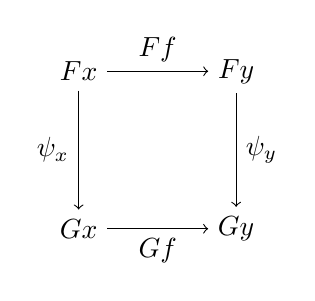
\begin{tikzpicture}
                    \node (FX) at (0, 0) {$Fx$};
                    \node (FY) at(2, 0) {$Fy$};
                    \node (GX) at (0, -2) {$Gx$};
                    \node (GY) at (2, -2) {$Gy$};
                    \draw[->] (FX) -- node[above]{$Ff$} (FY);
                    \draw[->] (GX) -- node[below]{$Gf$} (GY);
                    \draw[->] (FX) -- node[left]{$\psi_x$} (GX);
                    \draw[->] (FY) -- node[right]{$\psi_y$} (GY);
                \end{tikzpicture}
            \end{gather*}
        \end{enumerate}
    }
    \begin{definition}[Functor category]\index{functor!category}
        Consider two categories $\mathbf{A,B}$ where $\mathbf{A}$ is small. The functors $\func{F}{A}{B}$ form the objects of a category with the natural transformations as morphisms. This category is denoted by $\funccat{A}{B}$ or $\mathbf{B}^{\mathbf{A}}$ (the latter is a generalization of \ref{set:function_set}).
    \end{definition}

    \newdef{Dinatural transformation}{
        Consider two profunctors $\profunc{F,G}{A}{A}$ or, more generally, two functors $F,G:\mathbf{A}^{op}\times\mathbf{A}\rightarrow\mathbf{B}$. A dinatural transformation is a family of morphisms \[\eta_x:F(x,x)\rightarrow G(x,x)\] that make Diagram \ref{fig:dinatural} commute for every morphism $f:y\rightarrow x$.

        \begin{figure}[ht!]
            \centering
            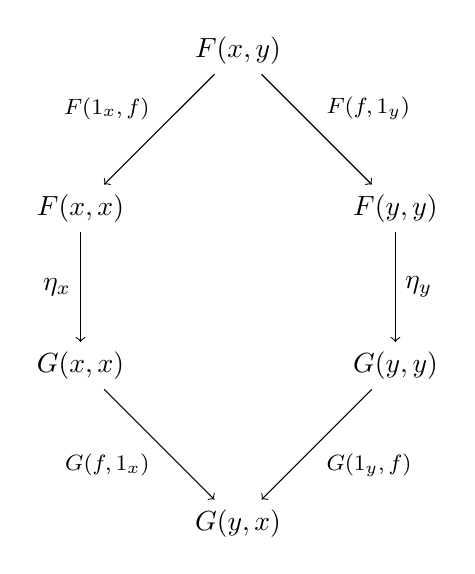
\begin{tikzpicture}
                \node (ab) at (0, 6) {$F(x,y)$};
                \node (F1) at (-2, 4) {$F(x,x)$};
                \node (F2) at (2, 4) {$F(y,y)$};
                \node (G1) at (-2, 2) {$G(x,x)$};
                \node (G2) at (2, 2) {$G(y,y)$};
                \node (ba) at (0, 0) {$G(y,x)$};

                \draw[->] (ab) edge node[above left]{\footnotesize$F(\mathbbm{1}_x,f)$} (F1) (F1) edge node[left]{$\eta_x$} (G1) (G1) edge node[below left]{\footnotesize$G(f,\mathbbm{1}_x)$} (ba);
                \draw[->] (ab) edge node[above right]{\footnotesize$F(f,\mathbbm{1}_y)$} (F2) (F2) edge node[right]{$\eta_y$} (G2) (G2) edge node[below right]{\footnotesize$G(\mathbbm{1}_y,f)$} (ba);
            \end{tikzpicture}
            \caption{Dinatural transformation.}
            \label{fig:dinatural}
        \end{figure}
    }

    \newdef{Representable functor}{\index{functor!representable}\index{representation}
        Let $\mathbf{C}$ be a locally small category. A functor $\func{F}{C}{Set}$ is said to be representable if there exists an object $x\in\ob{C}$ such that $F$ is naturally isomorphic to $h^x$. The pair $(x,\psi:F\Rightarrow h^x)$ is called a \textbf{representation} of $F$.
    }

    \begin{theorem}[Yoneda lemma]\index{Yoneda!lemma}
        Let $\mathbf{C}$ be a locally small category and let $\func{F}{C}{Set}$ be a functor. For every object $x\in\ob{C}$, there exists a natural isomorphism\footnote{Here, the fact that $\text{Nat}(h^-,-)$ can be seen as a functor $\mathbf{Set}^{\mathbf{C}}\times\mathbf{C}\rightarrow\mathbf{Set}$ is used.}
        \begin{gather}
            \eta_x:\text{\emph{Nat}}(h^x,F)\rightarrow Fx:\psi\mapsto\psi_x(\mathbbm{1}_x).
        \end{gather}
    \end{theorem}

    \begin{result}[Yoneda embedding]
        When $F$ is another hom-functor $h^y$, the following result is obtained:
        \begin{gather}
            \text{Nat}(h^x,h^y)\cong\mathbf{C}(y,x).
        \end{gather}
        Note that $y$ appears in the first argument on the right-hand side.

        Let $\mathbf{C}(f,-)$ denote the natural transformation corresponding to the morphism $f\in\mathbf{C}(y,x)$. The functor $h^-$, mapping an object $x\in\ob{C}$ to its hom-functor $\mathbf{C}(x,-)$ and a morphism $f\in\mathbf{C}(y,x)$ to the natural transformation $\mathbf{C}(f,-)$, can also be interpreted as a covariant functor $G:\mathbf{C}^{op}\rightarrow\mathbf{Set}^{\mathbf{C}}$. This way the Yoneda lemma can be seen to give rise to an embedding $h^-$ of $\mathbf{C}^{op}$ in the functor category $\mathbf{Set}^{\mathbf{C}}$.

        As usual, all of this can be done for contravariant functors. This gives an embedding
        \begin{gather}
            \mathcal{Y}:=h_-:\mathbf{C}\hookrightarrow\widehat{\mathbf{C}},
        \end{gather}
        called the Yoneda embedding.
    \end{result}

    \newdef{Local object}{\index{local!object}\label{cat:local_object}
        Consider a collection of morphisms $S\subset\text{hom}(\mathbf{C})$. An object $c\in\ob{C}$ is said to be $S$-local if the Yoneda embedding $\mathcal{Y}c$ maps morphisms in $S$ to isomorphisms in $\mathbf{Set}$. A morphism $f\in\text{hom}(\mathbf{C})$ is said to be $S$-local if its image under the Yoneda embedding of every $S$-local object is an isomorphism in $\mathbf{Set}$.
    }

\subsection{Equivalences}

    \newdef{Equivalence of categories}{\index{equivalence!of categories}
        Two categories $\mathbf{A},\mathbf{B}$ are said to be equivalent if there exist functors $\func{F}{A}{B}$ and $\func{G}{B}{A}$ such that $F\circ G$ and $G\circ F$ are naturally isomorphic to the identity functors.

        A weaker notion is that of a \textbf{weak equivalence}. Two categories $\mathbf{A},\mathbf{B}$ are said to be weakly equivalent if there exist functors $\func{F}{A}{B}$ and $\func{G}{B}{A}$ that are fully faithful and essentially surjective. Assuming the axiom of choice, every weak equivalence is also a (strong) equivalence (in fact this statement is equivalent to the axiom of choice).
    }

    \newdef{Skeletal category}{\index{category!skeletal}
        A category in which every isomorphism is necessarily an identity morphism. The \textbf{skeleton} of a category is an equivalent skeletal category (often taken to be a subcategory by choosing a representative from every isomorphism class).

        If one does not assume the axiom of choice, the skeleton is merely a \textit{weakly equivalent} skeletal category.
    }

    \newdef{Decategorification}{\index{decategorification}\label{cat:decategorification}
        Let $\mathbf{C}$ be an (essentially) small category. The set of isomorphism classes of $\mathbf{C}$ is called the decategorification of $\mathbf{C}$. This amounts to a functor $\func{\text{Decat}}{Cat}{Set}$.
    }

\subsection{Stuff, structure and property}\index{forgetful}

    To classify properties of objects and the \textit{forgetfulness} of functors, it is interesting to make a distinction between stuff, structure and property. Consider for example a group. This is a set (\textit{stuff}) equipped with a number of operations (\textit{structure}) that obey some relations (\textit{properties}).

    Using these notions one can classify forgetful functors in the following way:
    \begin{itemize}
        \item A functor forgets nothing if it is an equivalence of categories.
        \item A functor forgets at most properties if it is fully faithful.
        \item A functor forgets at most structure if it is faithful.
        \item A functor forgets at most stuff if it is just a functor.
    \end{itemize}

    ?? COMPLETE (see e.g. nLab or the paper ``Why surplus structure is not superfluous'' by Nicholas Teh et al.) ??

\subsection{Adjunctions}\index{adjunction}\label{section:adjunction}

    \newdef{Hom-set adjunction}{
        Let $\func{F}{A}{B}$ and $\func{G}{B}{A}$ be two functors. These functors form a (hom-set) adjunction $F\dashv G$ if the following isomorphism is natural in both $x$ and $y$:
        \begin{gather}
            \Phi_{x,y}:\mathbf{B}(Fx,y)\cong\mathbf{A}(x,Gy).
        \end{gather}
        The functor $F$ (resp. $G$) is called the left (resp. right) adjoint and the image of a morphism under either of the natural isomoprhisms is called the adjunct of the other morphism.\footnote{The terms ``adjunct'' and ``adjoint'' are sometimes used interchangeably (cf. French versus Latin).}.
    }
    \begin{notation}
        An adjunction $F\dashv G$ between categories $\mathbf{A,B}$ is often denoted by \[\mathbf{B}\adj{F}{G}\mathbf{A}.\]
    \end{notation}

    \newdef{Unit-counit adjunction}{\index{triangle!identities}\index{unit}\index{zig-zag|see{triangle identity}}\label{cat:unit_counit_adjunction}
        Let $\func{F}{A}{B}$ and $\func{G}{B}{A}$ be two functors. These functors form a unit-counit adjunction if there exist natural transformations
        \begin{align}
            \varepsilon:F\circ G\Rightarrow\mathbbm{1}_{\mathbf{B}}\\
            \eta:\mathbbm{1}_{\mathbf{A}}\Rightarrow G\circ F
        \end{align}
        such that the following compositions are identity morphisms:
        \begin{align}
            F\overset{F\eta}{\longrightarrow}FGF&\overset{\varepsilon F}{\longrightarrow}F\\
            G\overset{\eta G}{\longrightarrow}GFG&\overset{G\varepsilon}{\longrightarrow}G.
        \end{align}
        These identities are sometimes called the \textbf{triangle} or \textbf{zig-zag identities} (the latter results from the shape of the associated \textit{string diagram}). The transformations $\eta$ and $\varepsilon$ are called the \textbf{unit} and \textbf{counit} respectively.
    }

    \begin{property}[Equivalence of the above definitions]
        Every hom-set adjunction induces a unit-counit adjunction. Let $\Phi$ be the natural isomorphism associated to the hom-set adjunction $F\dashv G$. The counit $\varepsilon_y$ is obtained as the adjunct $\Phi^{-1}_{Gy,y}(\mathbbm{1}_{Gy})$ of the identity morphism on $Gy\in\ob{A}$, and the unit $\eta_x$ is analogously defined as the adjunct $\Phi_{c,Fc}(\mathbbm{1}_{Fx})$ of the identity morphism at $Fx\in\ob{B}$.

        Conversely, every unit-counit adjunction induces a hom-set adjunction. Consider a morphism $f:Fx\rightarrow y$. The (right) adjunct is defined as the composition \[\widetilde{f}:=Gf\circ\eta_x:x\rightarrow (G\circ F)x\rightarrow Gy.\] To construct a (left) adjunct, consider a morphism $\widetilde{g}:x\rightarrow Gy$: \[g:=\varepsilon_y\circ F\tilde{g}:Fx\rightarrow(F\circ G)y\rightarrow y.\]
    \end{property}

    \newdef{Reflective subcategory}{\index{category!reflective}\label{cat:reflective_inclusion}
        A full subcategory is said to be reflective (resp. coreflective) if the inclusion functor admits a left (resp. right) adjoint.
    }
    \begin{property}[Adjoint equivalence]\index{equivalence!adjoint}
        Any equivalence of categories is part of an adjoint equivalence, i.e. an adjunction for which the unit and counit morphisms are invertible.
    \end{property}

\section{General constructions}

    \newdef{Dagger category}{\index{category!dagger}\label{cat:dagger_category}
        A category equipped with a contravariant involutive endofunctor, this functor is often denoted by $\func{\dagger}{C}{C}$, similar to the adjoint operator for Hermitian matrices.
    }
    \begin{remark}\index{unitary}\index{self-adjoint}
        The concept of a dagger structure allows the usual definition of \textbf{unitary} and \textbf{self-adjoint} morphisms, i.e. morphism satisfying
        \begin{gather}
            f^\dagger = f^{-1}\qquad\text{or}\qquad f^\dagger = f.
        \end{gather}
    \end{remark}

    \newdef{Comma category}{\index{category!comma}
        Let $\mathbf{A},\mathbf{B}$ and $\mathbf{C}$ be three categories and let $\func{F}{A}{C}$ and $\func{G}{B}{C}$ be two functors. The comma category $F\downarrow G$ is defined as follows:
        \begin{itemize}
            \item\textbf{Objects}: The triples $(x,y,\gamma)$ where $x\in\ob{A},y\in\ob{B}$ and $\gamma:Fx\rightarrow Gy$.
            \item\textbf{Morphisms}: The morphisms $(x,y,\gamma)\rightarrow(k,l,\sigma)$ are pairs $(f,g)$ with $f:x\rightarrow k\in\text{hom}(\mathbf{A})$ and $g:y\rightarrow l\in\text{hom}(\mathbf{B})$ such that $\sigma\circ Ff = Gg\circ\gamma$.
            \item Composition of morphisms is defined componentwise.
        \end{itemize}
    }
    \newdef{Arrow category}{\index{category!arrow}\index{walking!arrow}\index{interval!category}
        The comma category of the pair of functors $(\mathbbm{1}_{\mathbf{C}},\mathbbm{1}_{\mathbf{C}})$. This is equivalently the functor category $[\mathbf{2},\mathbf{C}]$ where $\mathbf{2}$ is the \textbf{interval category/walking arrow} $\{0\rightarrow1\}$.
    }
    \newdef{Functorial factorization}{\index{factorization!functorial}\label{cat:functorial_factorization}
        A \textit{section} of the composition functor \[\func{\circ}{[3,C]}{[2,C]},\] where $\mathbf{3}$ is the poset $\{0\rightarrow1\rightarrow2\}$.
    }

    \newdef{Slice category}{\index{category!slice}
        Let $\mathbf{C}$ be a category and consider an object $x\in\ob{C}$. The slice category $\mathbf{C}/x$ of $\mathbf{C}$ over $x$ is defined as follows:
        \begin{itemize}
            \item\textbf{Objects}: The morphisms in $\mathbf{C}$ with codomain $x$.
            \item\textbf{Morphisms}: The morphisms $f\rightarrow g$ are morphisms $h$ in $\mathbf{C}$ such that $g\circ h = f$.
        \end{itemize}
        This category is also called the \textbf{over-category} of $x$. By dualizing one obtains the \textbf{under-category} of $x$.
    }

\subsection{\difficult{Fibred categories}}\label{section:fibred_categories}

    \newdef{Fibre category}{\index{fibre!category}\label{cat:fibre_category}
        Let $\func{\Pi}{A}{B}$ be a functor. The fibre category (of $\Pi$) over $y\in\ob{B}$ is the subcategory of $\mathbf{A}$ consisting of all objects $x\in\ob{A}$ such that $\Pi\,x=y$ and all morphisms $m\in\mathrm{hom}(\mathbf{A})$ such that $\Pi\,m=\mathbbm{1}_y$. It will be denoted by $\mathbf{A}_y$.

        Morphisms in $\mathbf{A}$ that are mapped to a morphism $f$ in $\mathbf{B}$ are called \textbf{$f$-morphisms} and, in particular (using the identification of objects and their identity morphisms), morphisms in $\mathbf{A}_y$ are called \textbf{$y$-morphisms}. Similarly, \textbf{$B$-categories} are defined as the categories equipped with a (covariant) functor to $\mathbf{B}$. (It is not hard to see that these form a \textit{2-category} under composition of functors that respects the $\mathbf{B}$-category structure.)
    }

    \newdef{Cartesian morphism}{\index{Cartesian!morphism}
        Consider a $\mathbf{B}$-category $\func{\Pi}{A}{B}$. A morphism $f$ in $\mathbf{A}$ is called $\Pi$-Cartesian if every $\Pi f$-morphism factors uniquely through a $y$-morphism, where $y$ is the domain of $\Pi f$.

        There also exists a notion of stronger notion. A \textbf{strongly Cartesian morphism} is a morphism $f\in\mathrm{hom}(\mathbf{A})$ such that for every morphism $\varphi\in\mathrm{hom}(\mathbf{A})$ with the same target and every factorization of $\Pi\varphi$ through $\Pi f$ there exists a unique factorization of $\varphi$ through $f$ that maps to the given factorization of $\Pi\varphi$.

        The following diagram (where the triangles commute) should clarify the above (technical) definitions:
        \begin{gather*}
            \begin{tikzpicture}
                \node (X3) at (0,2) {$\forall x'$};
                \node (X1) at (0,0) {$x_1$};
                \node (X2) at (2,0) {$x_2$};
                \node (arrow) at (4,1) {$\overset{\Pi}{\mapsto}$};
                \node (pX3) at (6,2) {$\Pi\,x'$};
                \node (pX1) at (6,0) {$\Pi\,x_1$};
                \node (pX2) at (8,0) {$\Pi\,x_2$};
                \draw[->] (X1) -- node[below]{$f$} (X2);
                \draw[->] (X3) -- node[left]{$\exists! g$} (X1);
                \draw[->] (X3) -- node[above right]{$\forall\varphi$} (X2);
                \draw[->] (pX1) -- node[below]{$\Pi f$} (pX2);
                \draw[->] (pX3) -- node[left]{$\forall \nu$} (pX1);
                \draw[->] (pX3) -- node[above right]{$\Pi\varphi$} (pX2);
            \end{tikzpicture}
        \end{gather*}
        The diagram for (weak) Cartesian morphisms is obtained by identifying the objects $\Pi\,x'$ and $\Pi\,x_1$, i.e. by restricting to the case $\nu=\mathbbm{1}_{\Pi x_1}$.

        The Cartesian morphisms are said to be \textbf{inverse images} of their projections under $\Pi$ and the object $x_1$ is called an \textbf{inverse image} of $x_2$ by $\Pi f$. The Cartesian morphisms of a fibre category are exactly the isomorphisms of that category.
    }

    \newdef{Fibred category}{\index{fibred!category}\index{Grothendieck!fibration|see{fibred category}}\index{fibration}
        A $\mathbf{B}$-category $\func{\Pi}{A}{B}$ is called a fibred category or \textbf{Grothendieck fibration} if the following conditions are satisfied:
        \begin{enumerate}
            \item Each morphism in $\mathbf{B}$ whose codomain lies in the range of $\Pi$ has at least one inverse image (in the weak sense).
            \item The composition of two Cartesian morphisms is again Cartesian (in the weak sense).
        \end{enumerate}
        If one instead works with strongly Cartesian morphisms, the second condition follows from the first one. However, it should be noted that in a fibred category a morphism is weakly Cartesian if and only if it is strongly Cartesian.
    }
    \newdef{Cleavage}{\index{cleavage}\index{cloven|see{cleavage}}
        Given a $\mathbf{B}$-category $\func{\Pi}{A}{B}$, a cleavage is the choice of a Cartesian $g$-morphism $f:x\rightarrow y$ for every $y\in\ob{A}$ and morphism $g:b\rightarrow \Pi\,a'$. A $\mathbf{B}$-category equipped with a cleavage is said to be \textbf{cloven}.

        It is clear that the existence of cleavage is sufficient for a category to be fibred and, conversely (assuming the axiom of choice), every fibred category admits a cleavage.
    }

    The following example can be obtained as a Grothendieck fibration with discrete fibres:
    \begin{example}[Discrete fibration]
        A functor $\func{F}{A}{B}$ such that for every object $x\in\ob{A}$ and every morphism $f:y\rightarrow Fx$ in $\mathbf{B}$ there exists a unique morphism $g:z\rightarrow x$ in $\mathbf{A}$ such that $Fg = f$.
    \end{example}
    \begin{example}[Groupoidal fibration]
        If every morphism is required to be Cartesian, the notion of a groupoid(al) fibration or a \textbf{category fibred in groupoids} is obtained. The reason for this name is that every fibre is a groupoid. An equivalent definition is that the associated pseudofunctor (see the construction below) factors through the embedding $\mathbf{Grpd}\hookrightarrow\mathbf{Cat}$.
    \end{example}

    \begin{property}[\difficult{Grothendieck construction}]\index{Grothendieck!construction}
        Every cloven category $\func{\Pi}{A}{B}$ defines a \textit{pseudofunctor}\footnote{See Definition \ref{cat:pseudofunctor} towards the end of this chapter.} $\cfunc{F}{B}{Cat}$ which sends objects to fibre categories and arrows $f$ to the pullback functor $f^*$ constructed from a Cartesian morphism covering $f$. Conversely, every pseudofunctor gives rise to a fibred category through the following construction. (These two constructions constitute a 2-equivalence of 2-categories.)

        The Grothendieck construction gives a (2-)functor $\int:\cfunccat{C}{Cat}\rightarrow\mathbf{Cat}/\mathbf{C}$. Consider a pseudofunctor $\cfunc{F}{C}{Cat}$. The ``bundle'' $\int\!F$ consists of the following data:
        \begin{itemize}
            \item The objects are pairs $(x,y)$ with $x\in\ob{C}$ and $y\in\mathrm{ob}(Fx)$.
            \item The morphisms $(x,y)\rightarrow(x',y')$ are pairs $(f:x\rightarrow x',\alpha:y\rightarrow Ff(y'))$.
        \end{itemize}
        Given a cleavage, the morphisms of the Grothendieck construction are exactly the factorizations of $f$-morphisms through the canonical lifting of $f$ in the cleavage.
    \end{property}
    \begin{property}[Functors]\index{split}
        A pseudofunctor is a functor if and only if the cleavage of the associated fibred category is \textbf{split(ting)}, i.e. it contains all identities and is closed under composition.
    \end{property}
    \begin{example}[Category of elements]\index{element}
        The Grothendieck construction applied to an ordinary presheaf $\cfunc{F}{C}{Set}$.
    \end{example}

\subsection{Monads}

    \newdef{Monad}{\index{monad}\label{cat:monad}
        A monad is a triple $(T,\mu,\eta)$ where $\func{T}{C}{C}$ is an endofunctor and $\mu:T^2\rightarrow T, \eta:\mathbbm{1}_{\mathbf{C}}\rightarrow T$ are natural transformations satisfying the following (coherence) conditions:
        \begin{enumerate}
            \item As natural transformations from $T^3$ to $T$:
            \begin{gather}
                \mu\circ T\mu = \mu\circ\mu_T.
            \end{gather}
            \item As natural transformations from $T$ to itself:
            \begin{gather}
                \mu\circ T\eta = \mu\circ\eta_T = \mathbbm{1}.
            \end{gather}
        \end{enumerate}
        These conditions say that a monad is a monoid \ref{algebra:monoid} in the category $\mathbf{End}_{\mathbf{C}}$ of endofunctors on $\mathbf{C}$. Accordingly, $\eta$ and $\mu$ are often called the \textbf{unit} and \textbf{multiplication} maps.
    }

    \begin{example}[Adjunction]
        Every adjunction $F\dashv G$, with unit $\varepsilon$ and counit $\eta$, induces a monad of the form $(GF,G\varepsilon F,\eta)$.
    \end{example}

    \newdef{Algebra over a monad\footnotemark}{\index{algebra!over a monad}\index{module}\label{cat:algebra_monad}
        \footnotetext{A more suitable name would be ``module over a monad'', since these are modules over a monoid if monads are regarded as monoids in $\mathbf{End}_{\mathbf{C}}$.}
        Consider a monad $(T,\mu,\eta)$ on a category $\mathbf{C}$. An algebra over $T$ is a couple $(x,\kappa)$, where $x\in\ob{C}$ and $\kappa:Tx\rightarrow x$, such that the following conditions are satisfied:
        \begin{enumerate}
            \item $\kappa\circ T\kappa = \kappa\circ\mu_x$, and
            \item $\kappa\circ\eta_x = \mathbbm{1}_x$.
        \end{enumerate}
        Morphisms $(x,\kappa_x)\rightarrow(y,\kappa_y)$ of $T$-algebras are morphisms $f:x\rightarrow y$ in $\mathbf{C}$ such that $f\circ\kappa_x = \kappa_y\circ Tf$. An algebra of the form $(Tx,\mu_x)$ is said to be \textbf{free}.
    }
    \newdef{Eilenberg-Moore category}{\index{Eilenberg-Moore category}
        Given a monad $T$ over a category $\mathbf{C}$, the Eilenberg-Moore category $\mathbf{C}^T$ is defined as the category of $T$-algebras.
    }
    \newdef{Kleisli category}{\index{Kleisli category}
        Consider a monad $T$ on a category $\mathbf{C}$. The Kleisli category $\mathbf{C}_T$ is defined as the full subcategory of $\mathbf{C}^T$ on the \textbf{free} $T$-algebras. This is equivalently the category with objects $\text{ob}(\mathbf{C}_T):=\ob{C}$ and morphisms $\mathbf{C}_T(x,y):=\mathbf{C}(x,Ty)$.
    }

    \newdef{Monadic adjunction}{\index{adjunction!monadic}
        An adjunction between categories $\mathbf{A}$ and $\mathbf{B}$ is said to be monadic if there exists an equivalence between $B$ and the Eilenberg-Moore category of the induced monad.
    }
    \newdef{Monadic functor}{\index{functor!monadic}
        A functor is said to be monadic if it admits a left adjoint such that the adjunction is monadic.
    }

    The following theorem characterizes monadic functors (for more information on some of the concepts, see Section \ref{section:morphisms} further below):
    \begin{theorem}[Beck's monadicity theorem]\index{Beck's monadicity theorem}
        Consider a functor $\func{F}{A}{B}$. This functor is monadic if and only if the following conditions are satisfied:
        \begin{itemize}
            \item $F$ admits a left adjoint.
            \item $F$ reflects isomorphisms, i.e. all morphims in the preimage of an isomorphism are also isomorphisms.
            \item $\mathbf{A}$ has all coequalizers of $F$-split parallel pairs\footnote{These are parallel pairs $f,g$ such that the images $Ff,Fg$ under $F$ admit a split coequalizer.} and $F$ preserves these coequalizers.
        \end{itemize}
    \end{theorem}
    \begin{remark}[Crude monadicity theorem]
        A sufficient condition for monadicity is obtained by replacing the third condition above by the following weaker statement: ``$\mathbf{A}$ has all coequalizers of reflexive pairs and $F$ preserves these coequalizers.''
    \end{remark}

    \newdef{Closure operator}{\index{closure!operator}\index{modal operator|see{closure operator}}\index{modal!type}\label{cat:closure_operator}
        Consider a monad $(\func{T}{C}{C},\eta,\mu)$. This monad is called a closure operator or \textbf{modal operator} if the multiplication map is a natural isomorphism, i.e. if the monad is idempotent.

        Given a closure operator $\func{T}{C}{C}$, the object $Tx$ is called the closure of $x\in\ob{C}$ and the associated morphism $\eta_x$ is called the \textbf{closing map}. $x\in\ob{C}$ itself is said to be $T$\textbf{-closed} exactly if its closing map is an isomorphism.

        An object $x\in\ob{C}$ is called a \textbf{modal type} if the unit $\eta_x:x\rightarrow Tx$ is an isomorphism.
    }

    \begin{remark}[\difficult{Bicategories}]
        A monad can be defined in any bicategory as a 1-morphism $t:x\rightarrow x$ together with two 2-morphisms that satisfy conditions similar to the ones above. The above definition is then just a specific case of this more general definition in the 2-category $\mathbf{Cat}$.

        In the general setting one can then also define a \textbf{module} over a monad. First of all, one can regard any object $x\in\ob{C}$ as a functor from the terminal category $1$. One can then replace $1$ by any other category in the ordinary definition to obtain a general algebra (or module) over a given monad. It is this definition that readily generalizes to bicategories, i.e. a module is a 1-morphism $a:x\rightarrow y$ together with a 2-morphism that satisfies the same conditions as an algebra over a monad in $\mathbf{Cat}$.
    \end{remark}

\section{Morphisms and diagrams}\label{section:morphisms}
\subsection{Morphisms}

    \newdef{Section}{\index{section}\index{retract}\label{cat:retract}
        A section of a morphism $f:x\rightarrow y$ is a right-inverse, i.e. a morphism $g:y\rightarrow x$ such that $f\circ g=\mathbbm{1}_y$. $f$ itself is called a \textbf{retraction} of $g$ and $y$ is called a \textbf{retract} of $x$.
    }

    \newdef{Monomorphism}{\index{monomorphism}
        Let $\mathbf{C}$ be a category. A morphism $\mu\in\mathbf{C}(x,y)$ is called a monomorphism, \textbf{mono} or \textbf{monic morphism} if for every object $z\in\ob{C}$ and every two morphisms $\alpha_1,\alpha_2\in\mathbf{C}(z,x)$ such that $\mu\circ\alpha_1 = \mu\circ\alpha_2$ one can conclude that $\alpha_1=\alpha_2$.
    }
    \newdef{Epimorphism}{\index{epimorphism}
        Let $\mathbf{C}$ be a category. A morphism $\varepsilon\in\mathbf{C}(x,y)$ is called an epimorphism, \textbf{epi} or \textbf{epic morphism} if for every object $z\in\ob{C}$ and every two morphisms $\alpha_1,\alpha_2\in\mathbf{C}(y,z)$ such that $\alpha_1\circ\varepsilon = \alpha_2\circ\varepsilon$ one can conclude that $\alpha_1=\alpha_2$.
    }

    \newdef{Split monomorphism}{\index{split}
        A morphism $f:x\rightarrow y$ that is a section of some other morphism $g:y\rightarrow x$. It can be shown that every split mono is in fact a mono and even an \textbf{absolute mono}, i.e. it is preserved by all functors.

        The morphism $g$ can be seen to satisfy the dual condition and hence is called a \textbf{split epimorphism}. It can be shown to be an absolute epi.
    }

    \newdef{Balanced category}{\index{category!balanced}\label{cat:balanced}
        A category in which every monic epi is an isomorphism.
    }

    \newdef{Reflexive pair}{
        Two parallel morphisms $f,g:x\rightarrow y$ are said to form a reflexive pair if they have a common section, i.e. if there exists a morphism $\sigma:y\rightarrow x$ such that $f\circ\sigma=g\circ\sigma=\mathbbm{1}_y$.
    }

    \newdef{Subobject}{\index{subobject}
        Let $\mathbf{C}$ be a category and let $x\in\ob{C}$ be any object. A subobject $y$ of $x$ is a mono $y\hookrightarrow x$.

        In fact, one should work up to isomorphisms and, accordingly, the formal definition goes as follows. A subobject $y$ of $x$ in the category $\mathbf{C}$ is an isomorphism class of monos $i:y\hookrightarrow x$ in the slice category $\mathbf{C}/x$.
    }
    \newdef{Well-powered category}{\index{well!powered}
        A category $\mathbf{C}$ is said to be well-powered if for every object $x\in\ob{C}$ the class of subobjects $\text{Sub}(x)$ is small.
    }

\subsection{Initial and terminal objects}

    \newdef{Initial object}{
        An object $\emptyset$ such that for every other object $x$ there exists a unique morphism $\iota_x:\emptyset\rightarrow x$.
    }
    \newdef{Terminal object}{
        An object $1$ such that for every other object $x$ there exists a unique morphism $\tau_x:x\rightarrow 1$.
    }
    \begin{property}[Uniqueness]
        If an initial (or terminal) object exists, it is unique (up to isomorphisms).
    \end{property}

    \newdef{Zero object}{\index{zero!object}\label{cat:zero_object}
        An object that is both initial and terminal. The zero object is often denoted by $0$.
    }
    \begin{property}[Zero morphism]
        From the definition of the zero object it follows that for any two objects $x,y$ there exists a unique morphism $0_{xy}:x\rightarrow0\rightarrow y$.
    \end{property}
    \newdef{Pointed category}{\index{pointed!category}\label{cat:pointed_category}
        A category containing a zero object.
    }

    \newdef{Global element}{\index{global!element}\label{cat:global_element}
        Let $\mathbf{C}$ be a category with a terminal object $1$. A global element of an object $x\in\ob{C}$ is a morphism $1\rightarrow x$.
    }
    \begin{property}
        Every global element is monic.
    \end{property}
    \newdef{Pointed object}{\index{pointed!object}
        An object $x$ equipped with a global element $1\rightarrow x$. This morphism is sometimes called the \textbf{basepoint}.
    }

    \begin{remark}\label{cat:global_elements_remark}
        In the category $\mathbf{Set}$ the elements of a set $S$ are in one-to-one correspondence with the global elements of $S$. Furthermore, there is the the important property (\textit{axiom of functional extensionality}) that two functions $f,g:S\rightarrow S'$ coincide if their values at every element $s\in S$ coincide or, equivalently, if their precompositions with global elements coincide.

        However, this way of checking equality can fail in other categories. Consider for example $\mathbf{Grp}$, the category of groups, with its zero object $0=\{e\}$. The only morphism from this group to any other group $G$ is the one mapping $e$ to the unit in $G$. It is obvious that precomposition with this morphism says nothing about the equality of other morphisms. To recover the extensionality property from $\mathbf{Set}$, the notion of an ``element'' should be generalized:
    \end{remark}
    \newdef{Generalized element}{\index{shape}
        Let $\mathbf{C}$ be category and consider an object $x\in\ob{C}$. For any object $y\in\ob{C}$, a morphism $y\rightarrow x$ is called a generalized element of $x$. They are also called \textbf{$y$-elements} in $x$ or elements of \textbf{shape} $y$ in $x$.
    }

    \newdef{Generator}{\index{generator}\index{separator|see{generator}}\label{cat:generator}
        Let $\mathbf{C}$ be a category. A collection of objects $\mathcal{O}\subset\ob{C}$ is called a collection of generators or \textbf{separators} for $\mathbf{C}$ if the generalized elements of shape $\mathcal{O}$ are sufficient to distinguish between all morphisms in $\mathbf{C}$:
        \begin{gather}
            \forall x,y\in\ob{C},\forall f,g\in\mathbf{C}(x,y):\Big(f\neq g\implies\exists o\in\mathcal{O},\exists h\in\mathbf{C}(o,x): f\circ h\neq g\circ h\Big).
        \end{gather}
    }
    \newdef{Well-pointed category}{\index{well!pointed}
        A category for which the terminal object is a generator.
    }

\subsection{Lifts}

    \newdef{Lifts and extensions}{\index{lift}\index{extension}
        A lift of a morphism $f:x\rightarrow y$ along an epi $e:z\rightarrow y$ is a morphism $g:x\rightarrow z$ satisfying $f=e\circ g$. Dualizing this definition gives the notion of extensions. (The epi/mono condition is often dropped in the literature.)
    }
    \newdef{Lifting property}{\index{orthogonal!lifting}\label{cat:lifting_property}
        A morphism $f:x\rightarrow y$ has the left lifting property with respect to a morphism $g:x'\rightarrow y'$ (or $g$ has the right lifting property with respect to $f$) if for every commutative diagram
        \begin{gather*}
            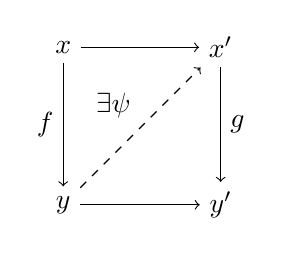
\begin{tikzpicture}
                \node (A) at (0, 0) {$x$};
                \node (B) at (0, -2) {$y$};
                \node (C) at (2, 0) {$x'$};
                \node (D) at (2, -2) {$y'$};
                \draw[->] (A) -- node[left]{$f$} (B);
                \draw[->] (A) -- (C);
                \draw[->, dashed] (B) -- node[above left]{$\exists\psi$} (C);
                \draw[->] (B) -- (D);
                \draw[->] (C) -- node[right]{$g$} (D);
            \end{tikzpicture}
        \end{gather*}
        there exists a morphism $\psi:y\rightarrow x'$ such that the triangles commute. If the morphism $\psi$ is unique, then $f$ and $g$ are said to be \textbf{orthogonal}.
    }
    \newdef{Injective and projective morphisms}{\index{injective!morphism}\index{projective!morphism}
        Consider a class of morphisms $I\subseteq\text{hom}(\mathbf{C})$. A morphism $f\in\text{hom}(\mathbf{C})$ is said to be $I$-injective (resp. $I$-projective) if it has the right (resp. left) lifting property with respect to all morphisms in $I$.

        Given a set of morphisms $I$, the sets of $I$-injective and $I$-projective morphisms are denoted by $\text{rlp}(I)$ and $\text{llp}(I)$, respectively.
    }
    \newdef{Injective and projective objects}{\index{injective!object}\index{projective!object}
        If $\mathbf{C}$ has a terminal object $1$, an object $x$ is called $I$-injective if its terminal morphism is $I$-injective. If $\mathbf{C}$ has an initial object, $I$-projective objects can be defined dually. (See Figure \ref{fig:inj_proj}.)

        \begin{figure}[ht!]
            \centering
            \begin{subfigure}[b]{0.49\textwidth}
                \centering
                \begin{tikzpicture}
                    \node (X) at (0, 0) {$x$};
                    \node (Y) at (0, -2) {$y$};
                    \node (C) at (2, 0) {$i$};
                    \draw[->] (X) -- node[left]{$\forall f\in I$} (Y);
                    \draw[->] (X) -- node[above]{$g$} (C);
                    \draw[dashed, ->] (Y) -- node[below right]{$\exists\psi$} (C);
                \end{tikzpicture}
                \caption{Injective object $i$.}
                \label{fig:injective_object}
            \end{subfigure}
            \begin{subfigure}[b]{0.49\textwidth}
                \centering
                \begin{tikzpicture}
                    \node (X) at (2, 2) {$x$};
                    \node (Y) at (2, 0) {$y$};
                    \node (C) at (0, 0) {$p$};
                    \draw[->] (X) -- node[right]{$\forall f\in I$} (Y);
                    \draw[->] (C) -- node[below]{$g$} (Y);
                    \draw[dashed, ->] (C) -- node[above left]{$\exists\psi$} (X);
                \end{tikzpicture}
                \caption{Projective object $p$.}
                \label{fig:projective_object}
            \end{subfigure}
            \caption{Injective and projective objects.}
            \label{fig:inj_proj}
        \end{figure}
        If $I$ is the class of monomorphisms (resp. epimorphisms), the terminology is simplified to \textbf{injective} (resp. \textbf{projective}) objects. For projective objects this is also equivalent to requiring that the (covariant) hom-functor preserves epimorphisms.

        A category $\mathbf{C}$ is said to \textbf{have enough injectives} if for every object there exists a monomorphism into an injective object. The category is said to \textbf{have enough projectives} if for every object there exists an epimorphism from a projective object.
    }
    \newdef{Fibrations and cofibrations}{\index{fibration}
        Consider a category $\mathbf{C}$ together with a class $I\subseteq\text{hom}(\mathbf{C})$ of morphisms. A morphism $f\in\text{hom}(\mathbf{C})$ is called an $I$-fibration (resp. $I$-cofibration) if it has the right (resp. left) lifting property with respect to all $I$-projective (resp. $I$-injective) morphisms.
    }

\subsection{Limits and colimits}\label{section:diagrams}

    \newdef{Diagram}{\index{diagram}
        A diagram in $\mathbf{C}$ with index category $\mathbf{I}$ is a (covariant) functor $\func{D}{I}{C}$.
    }

    \newdef{Cone}{\index{cone}
        Let $\func{D}{I}{C}$ be a diagram. A cone from $c\in\ob{C}$ to $D$ consists of a family of morphisms $\psi_i:c\rightarrow Di$ indexed by $\mathbf{I}$ such that $\psi_j = Df\circ\psi_i$ for all morphisms $f:i\rightarrow j\in\text{hom}(\mathbf{I})$. This is depicted in Figure \ref{fig:cone_component}.

        \begin{figure}[ht!]
            \centering
            \begin{subfigure}[b]{0.49\textwidth}
                \centering
                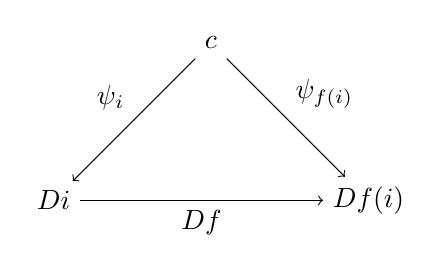
\begin{tikzpicture}
                    \node (1) at (0, 0) {$c$};
                    \node (2) at (-2, -2) {$Di$};
                    \node (3) at (2, -2) {$Df(i)$};
                    \draw[->] (1) -- node[above left]{$\psi_i$} (2);
                    \draw[->] (1) -- node[above right]{$\psi_{f(i)}$} (3);
                    \draw[->] (2) -- node[below]{$Df$} (3);
                \end{tikzpicture}
                \caption{Component of cone over $D$.}
                \label{fig:cone_component}
            \end{subfigure}
            \begin{subfigure}[b]{0.49\textwidth}
                \centering
                \begin{tikzpicture}
                    \node (1) at (0, -2) {$Di$};
                    \node (2) at (-2, 0) {$a$};
                    \node (3) at (2, 0) {$b$};
                    \draw[<-] (1) -- node[below left]{$\psi_i$} (2);
                    \draw[<-] (1) -- node[below right]{$\phi_i$} (3);
                    \draw[->] (2) -- node[above]{$f$} (3);
                \end{tikzpicture}
                \caption{Morphism of cones.}
                \label{fig:cone_morphism}
            \end{subfigure}
            \caption{Category of cones.}
            \label{fig:cone}
        \end{figure}
    }
    \begin{adefinition}\index{diagonal!functor}
        The above definition can be reformulated by defining an additional functor $\Delta_x:\mathbf{I}\rightarrow\mathbf{C}$ that maps every element $i\in\ob{I}$ to $x$ and every morphism $g\in\text{hom}(\mathbf{I})$ to $\mathbbm{1}_x$, i.e. $\Delta:C\rightarrow[\mathbf{I},\mathbf{C}]$ is the \textbf{diagonal functor}. The morphisms $\psi_i$ can then be seen to be the components of a natural transformation $\psi:\Delta_x\Rightarrow D$. Hence, a cone $(x,\psi)$ is an element of $[\mathbf{I},\mathbf{C}](\Delta_x,D)$.
    \end{adefinition}
    \newdef{Morphism of cones}{\index{morphism!of cones}
        Let $\func{D}{I}{C}$ be a diagram and let $(x,\psi)$ and $(y,\phi)$ be two cones over $D$. A morphism between these cones is a morphism of the apexes $f:x\rightarrow y$ such that the diagrams of the form \ref{fig:cone_morphism} commute for all $i\in\ob{I}$. The cones over $D$ together with these morphisms form a category $\mathbf{Cone}(D)$, in fact this can easily be seen to be the comma category $\Delta\downarrow D$.
    }

    \newdef{Limit}{\index{limit}
        Consider a diagram $\func{D}{I}{C}$. The limit of this diagram, denoted by $\lim D$, is (if it exists) the terminal object of the category $\mathbf{Cone}(D)$.
    }
    \begin{remark*}\index{projective!limit}\index{inductive!limit}
        In the older literature the name \textbf{projective limit} was sometimes used. The dual notion, a \textbf{colimit}, is often called an \textbf{inductive limit} in the older literature.
    \end{remark*}
    This definition leads to the following universal property:
    \begin{uproperty}\label{cat:limit_uproperty}
        Let $\func{D}{I}{C}$ be a diagram. For every cone $(x,\psi)\in\mathbf{Cone}(D)$, there exists a unique morphism $f:x\rightarrow\lim D$. This defines a bijection \[[\mathbf{I}, \mathbf{C}](\Delta_x,D)\cong\mathbf{C}(x,\lim D).\]
        If all (small) limits exist, the limit functor $\func{\lim}{[I,C]}{C}$ can be defined. The universal property of limits then implies that it is right adjoint to the constant functor $\Delta$.

        For diagrams in $\mathbf{Set}$ one can use the fully faithfulness of the Yoneda embedding to obtain the following expression:
        \begin{gather}
            \lim D\cong\funccat{I}{Set}(\Delta_\ast,D).
        \end{gather}
    \end{uproperty}
    \begin{remark}
        In Section \ref{section:enriched_category_theory} on enriched category theory, a generalization (the so-called \textit{weighted limits}) of the above construction will be given that is better suited to the enriched setting and allows to express a wide variety of constructions as (weighted) limits.
    \end{remark}

    \begin{example}[Terminal object]
        The terminal object $1$ is the limit of the empty diagram.
    \end{example}

    \newdef{Finitely complete category}{\index{category!complete}
        A category is said to be finitely complete if it has all finite limits. If all (small) limits exist, the category is said to be \textbf{complete}. The dual notion for colimits is called \textbf{(finite) cocompleteness}.
    }
    \begin{example}[Presheaf categories]\label{cat:complete_presheaf_category}
        All presheaf categories are both complete and cocomplete.
    \end{example}

    \newdef{Continuous functor}{\index{continuity!functor}\label{cat:continuity}
        A functor that preserves all small limits.
    }
    \begin{example}[Hom-functors]
        In a locally small category every hom-functor is continuous (in fact these functors even preserve limits that are not necessarily small). This implies for example that
        \begin{gather}
            \mathbf{C}(x,\lim D)\cong\lim\mathbf{C}(x, D).
        \end{gather}
    \end{example}

    In the case where $\mathbf{C}$ is small, one can characterize the Yoneda embedding through a universal property:
    \begin{uproperty}[Free cocompletion]\index{co-!completion}\index{Yoneda!embedding}\label{cat:free_cocompletion}
        The Yoneda embedding $\mathbf{C}\hookrightarrow\widehat{\mathbf{C}}$ turns the presheaf category $\widehat{\mathbf{C}}$ into the \textbf{free cocompletion} of $\mathbf{C}$, i.e. there exists an equivalence of categories between the functor category of cocontinuous functors $[\widehat{\mathbf{C}},\mathbf{D}]_{\text{cont}}$ and the ordinary functor category $[\mathbf{C},\mathbf{D}]$.
    \end{uproperty}

    \newdef{Tiny object}{\index{tiny}\label{cat:tiny}
        An object in a locally small category for which the covariant hom-functor preserves small colimits. This is sometimes called a \textbf{small-projective} object since it is in particular projective\footnote{Epimorphisms are characterized by a \textit{pushout} (see \ref{cat:pushout_epi} further below).}.
    }
    \newdef{Cauchy completion}{\index{Cauchy!completion}\index{Karoubi!envelope}
        Let $\mathbf{C}$ be a small category. An important (small and full) subcategory of the free cocompletion of $\mathbf{C}$ is given by the Cauchy completion, i.e. the subcategory of $\widehat{\mathbf{C}}$ on the tiny objects.\footnote{A generalization in the context of enriched categories is given by the \textit{Karoubi envelope}.} It can be shown that the free cocompletion of the Cauchy completion coincides with the one on $\mathbf{C}$ (up to equivalence).

        A category is said to be \textbf{Cauchy-complete} if it is equivalent to its Cauchy completion. It can be shown that a category is Cauchy-complete if and only if it has all small absolute colimits.
    }

    \newdef{Filtered category}{\index{category!filtered}
        A category in which every finite diagram admits a cocone. For regular cardinals $\kappa$, this notion can be generalized. A category is said to be $\kappa$-filtered if every diagram with less than $\kappa$ arrows admits a cocone. (In this terminology filtered categories are the same as $\omega$-filtered categories.)
    }

    \newdef{Directed limit}{\index{limit!directed}
        Consider a diagram $\func{D}{I}{C}$. The limit (resp. colimit) of $D$ is said to be codirected (resp. directed) if $\mathbf{I}$ is a downward (resp. upward) directed set \ref{set:directed_set}.
    }
    The following definition is a categorification of the previous one:
    \newdef{Filtered limit}{\index{limit!filtered}
        Consider a diagram $\func{D}{I}{C}$. The limit (resp. colimit) of $D$ is said to be cofiltered (resp. filtered) if $\mathbf{I}$ is a cofiltered (resp. filtered) category.
    }
    \begin{property}\label{cat:directed_filtered}
        A category has all directed colimits if and only if it has all filtered colimits. (A dual statement holds for limits.)
    \end{property}

    \newdef{Pro-object}{\index{pro!object}
        A functor $\func{F}{I}{C}$ where $\mathbf{I}$ is a small cofiltered category. The names stems from the fact that one can interpret pro-objects as formal cofiltered (projective) limits.
    }

    \newdef{Compact object}{\index{compact}\index{presentable}
        An object for which the covariant hom-functor preserves all filtered colimits. These objects are also said to be \textbf{finitely presentable}.\footnote{This name derives from the fact that modules are finitely presented if and only if their covariant hom-functor preserves direct limits (i.e. directed colimits in the context of algebra).}
    }

    \newdef{Product}{\index{product}\index{co-!product}\label{cat:product}
        Let $\mathbf{I}$ be a discrete category. The (co)limit over a diagram $\func{D}{I}{C}$ is called a (co)product in $\mathbf{C}$.
    }

    \newdef{Equalizer}{\index{equalizer}\index{fork}
        Consider a diagram of the form \[x\overset{f}{\underset{g}{\rightrightarrows}}y.\] The limit of this diagram is called the equalizer of $f$ and $g$. It consists of an object $e$ and a morphism $\varepsilon:e\rightarrow x$ such that the following \textbf{fork} diagram
        \begin{gather}
            e\overset{\varepsilon}{\rightarrow}x\overset{f}{\underset{g}{\rightrightarrows}} y
        \end{gather}
        is universal with respect to $(e,\varepsilon)$. By dualizing one obtains \textbf{cofork} diagrams $x\rightrightarrows y\rightarrow z$ and their universal versions, the \textbf{coequalizers}.
    }
    \newdef{Split coequalizer}{\index{split}\label{cat:split_coequalizer}
        A cofork diagram \[x\overset{f}{\underset{g}{\rightrightarrows}}y\overset{\tau}{\rightarrow}z\] together with a section $\varphi$ of $f$ and a section $\sigma$ of $\tau$ such that $\sigma\circ\tau = g\circ\varphi$.
    }

    \newdef{Regular morphisms}{\index{regular!morphism}
        A mono (resp. epi) is said to be regular if it arises as an equalizer (resp. coequalizer) of two parallel morphisms.
    }
    \begin{property}[Regular bimorphism]\index{bimorphism}\label{cat:regular_iso}
        Both monic regular epimorphisms and epic regular monomorphisms are isomorphisms.
    \end{property}

    \newadef{Finitely complete category}{\index{category!complete}
        A category is said to be finitely complete if it has a terminal object and if all binary equalizers and products exist.
    }

    \newdef{Span}{\index{span}
        A span in a category $C$ is a diagram of the form \ref{fig:cat_span}. By definition of a diagram, a span in $C$ is equivalent to a functor $\func{S}{\Lambda}{C}$, where $\mathbf{\Lambda}$ is the category with three objects $\{-1,0,1\}$ and two morphisms $i:0\rightarrow -1$ and $j:0\rightarrow 1$. For this reason $\mathbf{\Lambda}$ is sometimes called the walking or universal span.

        \begin{figure}[!ht]
            \centering
            \begin{subfigure}[b]{0.49\textwidth}
                \centering
                \begin{tikzpicture}
                    \node (X) at (-2, 0) {$x$};
                    \node (S) at (0, 2) {$s$};
                    \node (Y) at (2, 0) {$y$};
                    \draw[->] (S) -- node[above left]{$f$} (X);
                    \draw[->] (S) -- node[above right]{$g$} (Y);
                \end{tikzpicture}
                \caption{Span (category theory).}
                \label{fig:cat_span}
            \end{subfigure}
            \begin{subfigure}[b]{0.49\textwidth}
                \centering
                \begin{tikzpicture}
                    \node (X) at (-2, 2) {$x$};
                    \node (S) at (0, 0) {$c$};
                    \node (Y) at (2, 2) {$y$};
                    \draw[<-] (S) -- node[below left]{$f$} (X);
                    \draw[<-] (S) -- node[below right]{$g$} (Y);
                \end{tikzpicture}
                \caption{Cospan.}
                \label{fig:pullback}
            \end{subfigure}
            \caption{(Co)span diagrams.}
        \end{figure}
    }

    \newdef{Pullback}{\index{pullback}\index{fibre!product|seealso{pullback}}\index{Cartesian!square}\label{cat:pullback}
        The pullback or \textbf{fibre product} of two morphisms $f:x\rightarrow z$ and $g:y\rightarrow z$ is defined as the limit of cospan \ref{fig:pullback}. The full diagram characterizing the pullback, which has the form of a square, is sometimes called a \textbf{Cartesian square}.
    }
    \begin{notation}[Pullback]
        The pullback of two morphisms $f:x\rightarrow z$ and $g:y\rightarrow z$ is often denoted by $x\times_zy$. The associated pullback square is sometimes written as in Figure \ref{fig:pullback_square}.

        \begin{figure}[ht!]
            \centering
            \begin{subfigure}[b]{0.49\textwidth}
                \centering
                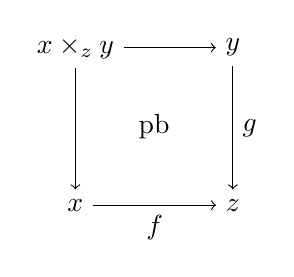
\begin{tikzpicture}
                    \node (X) at (0, -2) {$x$};
                    \node (Y) at (2, 0) {$y$};
                    \node (Z) at (2, -2) {$z$};
                    \node (pull) at (0, 0) {$x\times_zy$};
                    \node at (1, -1) {pb};
                    \draw[<-] (Z) -- node[below]{$f$} (X);
                    \draw[<-] (Z) -- node[right]{$g$} (Y);
                    \draw[->] (pull) -- (X);
                    \draw[->] (pull) -- (Y);
                \end{tikzpicture}
                \caption{Pullback square.}
                \label{fig:pullback_square}
            \end{subfigure}
            \begin{subfigure}[b]{0.49\textwidth}
                \centering
                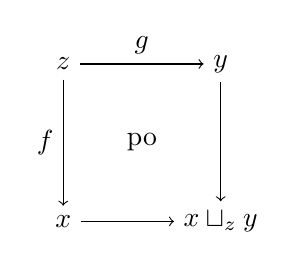
\begin{tikzpicture}
                    \node (X) at (0, -2) {$x$};
                    \node (Y) at (2, 0) {$y$};
                    \node (Z) at (0, 0) {$z$};
                    \node (push) at (2, -2) {$x\sqcup_zy$};
                    \node at (1, -1) {po};
                    \draw[->] (Z) -- node[left]{$f$} (X);
                    \draw[->] (Z) -- node[above]{$g$} (Y);
                    \draw[<-] (push) -- (X);
                    \draw[<-] (push) -- (Y);
                \end{tikzpicture}
                \caption{Pushout square.}
                \label{fig:pushout_square}
            \end{subfigure}
            \caption{Pullback and pushout diagrams.}
        \end{figure}
    \end{notation}

    \begin{property}[Product]\index{product}
        If a terminal object $1$ exists, the pullback $x\times_1y$ is equal to the product $x\times y$.
    \end{property}
    \newdef{Kernel pair}{\index{kernel}
        Consider a morphism $f:x\rightarrow y$. Its kernel pair is defined as the pullback of $f$ along itself.
    }

    \newdef{Pushout}{\index{pushout}\label{cat:pushout}
        The dual notion of a pullback, i.e. the colimit of a span. See Figure \ref{fig:pushout_square}.
    }

    \begin{property}
        Pullbacks preserve monos and pushouts preserve epis.
    \end{property}
    \newadef{Epimorphism}{\index{epimorphism}\label{cat:pushout_epi}
        A morphism whose cokernel pair is the identity.
    }

    \begin{property}[\difficult{Span category}]\label{cat:span_category}
        \nomenclature[S_span]{$\mathbf{Span}(\mathbf{C})$}{span category over $\mathbf{C}$}
        Consider a category $\mathbf{C}$ with pullbacks. The category $\mathbf{Span}(\mathbf{C})$ is defined as the category with the same objects as $\mathbf{C}$ but with spans as morphisms. Composition of spans is given by pullbacks. By including morphisms of spans, $\mathbf{Span}(\mathbf{C})$ can be refined to a bicategory.
    \end{property}

    \newdef{Wedge}{\index{wedge}
        Consider a profunctor $\profunc{F}{C}{C}$. A wedge $e:w\rightarrow F$ is an object $w\in\ob{Set}$ together with a collection of morphisms $e_x:w\rightarrow F(x,x)$ indexed by $\mathbf{C}$ such that for every morphism $f:x\rightarrow y$ the following diagram commutes:
        \begin{gather*}
            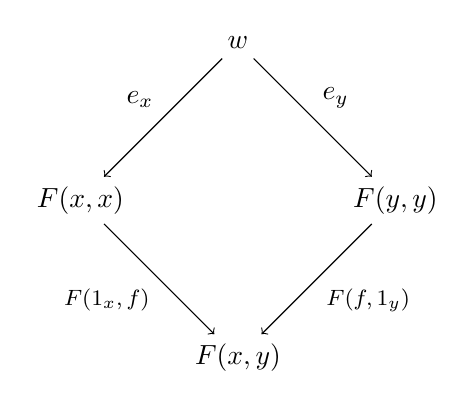
\begin{tikzpicture}
                \node (W) at (0, 4) {$w$};
                \node (F1) at (-2, 2) {$F(x,x)$};
                \node (F2) at (2, 2) {$F(y,y)$};
                \node (F) at (0, 0) {$F(x,y)$};
                \draw[->] (W) edge node[above left]{$e_x$} (F1) (F1) edge node[below left]{\footnotesize$F(\mathbbm{1}_x,f)$} (F);
                \draw[->] (W) edge node[above right]{$e_{y}$} (F2) (F2) edge node[below right]{\footnotesize$F(f,\mathbbm{1}_{y})$} (F);
            \end{tikzpicture}
        \end{gather*}
        As was the case for cones, this can be reformulated in terms of (di)natural transformations. A wedge $(w,e)$ of a profunctor $\profunc{F}{C}{C}$ is a dinatural transformation from the constant profunctor $\Delta_w$ to $F$.
    }
    \newdef{End}{\index{end}
        The end of a profunctor $\profunc{F}{C}{C}$ is defined as the universal wedge of $F$. The components of the wedge are called the \textbf{projection maps} of the end. This stems from the fact that for a discrete category the end coincides with the product $\prod_{x\in\ob{C}}F(x,x)$.

        This is equivalent to a definition in terms of equalizers. Consider the two canonical maps \[\prod_{x\in\ob{C}}\mathbf{C}(x,x)\rightrightarrows\prod_{f:x\rightarrow y}\mathbf{C}(x,y).\] This diagram can be interpreted as the product of all lower halves of the wedge diagrams above. It is not hard to see that its equalizer (universally) satisfies the wedge condition for all $f\in\text{hom}(\mathbf{C})$.
    }
    \newnot{End}{
        The end of a profunctor $\profunc{F}{C}{C}$ is often denoted using an integral sign with subscript: \[\int_{x\in\mathbf{C}}F(x,x).\] For the dual construction, called a \textbf{coend}, an integral sign with superscript is used.
    }
    \begin{example}[Natural transformations]\index{natural!transformation}
        Consider two functors $\func{F,G}{A}{B}$. The map $(x,y)\mapsto\mathbf{B}(Fx,Gy)$ gives a profunctor $\profunc{H}{A}{A}$. By looking at the wedge condition for this profunctor, the following equality for all morphisms $f:x\rightarrow y$ can be derived:
        \begin{gather}
            \tau_y\circ Ff = Gf\circ\tau_x,
        \end{gather}
        where $\tau$ is the wedge projection. Comparing this equality to Definition \ref{cat:natural} gives
        \begin{gather}
            \label{cat:natural_end}
            \text{Nat}(F,G) = \int_{x\in\mathbf{A}}\mathbf{B}(Fx,Gx).
        \end{gather}
    \end{example}

    \begin{property}
        Using the continuity \ref{cat:continuity} of the hom-functor, one can prove the following equality which can be used to turn ends into coends and vice versa:
        \begin{gather}
            \mathbf{Set}\left(\int^{x\in\mathbf{C}}F(x,x),y\right) = \int_{x\in\mathbf{C}}\mathbf{Set}\left(F(x,x),y\right).
        \end{gather}
    \end{property}

    Using the above properties and definitions, one obtains the following two statements, called the \textbf{Yoneda reduction} and \textbf{co-Yoneda lemma}:
    \begin{property}[Ninja Yoneda lemma]\index{Yoneda!lemma}\label{cat:ninja_yoneda}
        Let $\func{F}{A}{B}$ be a covariant functor (similar statements hold for contravariant functors).
        \begin{align}
            &\int_{x\in\mathbf{A}}\mathbf{Set}\left(\mathbf{A}(-,x),Fx\right)\cong F\\
            &\int^{x\in\mathbf{A}}\mathbf{A}(x,-)\times Fx\cong F.
        \end{align}
        For a generalization to the enriched setting see Definition \ref{cat:enriched_kan_extension}.
    \end{property}
    \begin{remark}
        A common remark at this point is the comparison with the Dirac distribution \ref{distribution:sieving_dirac_delta}:
        \begin{gather}
            \int \delta(x-y)f(x) = f(y).
        \end{gather}
        By interpreting the functor $F$ as a function, the representable functors can be seen to behave as Dirac distributions.
    \end{remark}

    \begin{property}
        \begin{gather}
            \int_{F\in\mathbf{coPsh}(\mathbf{C})}\mathbf{Set}(Fx,Fy)\cong\mathbf{C}(x,y)
        \end{gather}
    \end{property}


    \newdef{Kan extension}{\index{Kan!extension}\label{cat:kan_extension}
        Consider two functors $\func{F}{A}{B}$ and $\func{G}{A}{C}$. The right Kan extension of $F$ along $G$ is given by the universal functor $\func{\mathrm{Ran}_GF}{C}{B}$ and natural transformation $\eta:\mathrm{Ran}_GF\circ G\Rightarrow F$:
        \begin{gather*}
            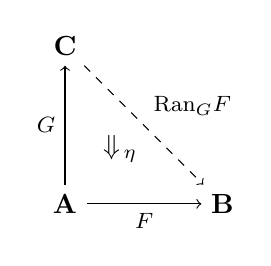
\begin{tikzpicture}
                \node (A) at (0, 0) {$\mathbf{A}$};
                \node (B) at (2, 0) {$\mathbf{B}$};
                \node (C) at (0, 2) {$\mathbf{C}$};
                \node at (0.7, 0.7) {$\Downarrow_{\,\eta}$};
                \draw[->] (A) -- node[left]{\footnotesize$G$} (C);
                \draw[->] (A) -- node[below]{\footnotesize$F$} (B);
                \draw[dashed, ->] (C) -- node[above right]{\footnotesize$\mathrm{Ran}_GF$} (B);
            \end{tikzpicture}
        \end{gather*}
        The left Kan extension $\mathrm{Lan}_GF$ is obtained by dualizing this construction.
    }

    \begin{property}[Complete categories]
        Complete (resp. cocomplete) categories admit all right (resp. left) Kan extensions.
    \end{property}

    \newdef{Preservation of Kan extension}{\label{cat:preservation_kan_extension}
        A Kan extension $\mathrm{Lan}_GF$ is said to be \textbf{absolute} if every functor with the same codomain as preserves the Kan extension, i.e. a Kan extension is absolute if right whiskering it by another functor defines the Kan extension of the composition. If it is only preserved by all representable functors,  the Kan extension is said to be \textbf{pointwise}.
    }

    \newadef{Kan extension}{
        The construction above gives a functor $\mathrm{Ran}_G$ from the functor category $\funccat{A}{B}$ to the functor category $\funccat{C}{B}$. The right Kan extension $\mathrm{Ran}_G$ can be defined as the right adjoint to the pullback functor $G^*:F\mapsto F\circ G$. Similarly, the left Kan extension can be defined as the left adjoint to the pullback functor.

        In the spirit of partial adjoints or partial limits, this definition can be used to define \textbf{local Kan extensions}. Although the left (or right) Kan extension functors do not have to exists globally, the extension of a single functor could still exist. This local version is defined by the following natural isomorphism (here given for a left extension):
        \begin{gather}
            \funccat{A}{B}(F,G^*-)\cong\funccat{C}{B}(\mathrm{Lan}_GF,-).
        \end{gather}
    }
    \remark{Using this equivalence of hom-spaces, Kan extensions can be generalized from $\mathbf{Cat}$ to any \textit{2-category}.}

    \begin{example}[Limit]\index{limit}
        Denote the terminal category by $\mathbf{1}$. By choosing the functor $G$ in the definition of a right Kan extension to be the unique functor $!_{\mathbf{C}}:\mathbf{C}\rightarrow\mathbf{1}$, one obtain the universal property characterizing limits \ref{cat:limit_uproperty}:
        \begin{gather}
            \lim F\cong\mathrm{Ran}_{!_C}F.
        \end{gather}
        Similarly, colimits can be obtained as left Kan extensions.
    \end{example}

    The existence of Kan extensions can also be used to determine the existence of adjoints:
    \begin{property}[Adjoint functors]
        A functor $\func{F}{A}{B}$ admits a left (resp. right) adjoint if and only if the right (resp. left) Kan extension of the identity functor $\func{\mathbbm{1}}{A}{A}$ along $F$ exists. If it exists as an absolute extension, the left adjoint is given exactly by this Kan extension.
    \end{property}

    \newdef{Codensity monad}{\index{monad!codensity}\index{co-!dense}
        Consider a general functor $\func{F}{A}{B}$. If the right Kan extension $\text{Ran}_FF$ exists, it defines a monad. Functors for which this monad is the identity are said to be \textbf{codense}.\footnote{Codense functors are usually defined in a different way, but one can show that this is an equivalent definition (hence the name).} Left Kan extensions give, by duality, rise to \textit{density comonads}.
    }

\section{Internal structures}\index{internal}

    \begin{property}[Eckmann-Hilton argument]\index{Eckmann-Hilton!argument}\label{cat:eckmann_hilton}
        A monoid internal to $\mathbf{Mon}$, the category of monoids is the same as a commutative monoid. (See also Property \ref{algebra:eckmann_hilton}.)
    \end{property}

    \newdef{Internal category}{\label{cat:internal_category}
        Let $\mathcal{E}$ be a category with pullbacks. A category $\mathbf{C}$ internal to $\mathcal{E}$ consists of the following data:
        \begin{itemize}
            \item an object $C_0\in\ob{\mathcal{E}}$ of objects;
            \item an object $C_1\in\ob{\mathcal{E}}$ of morphisms;
            \item source and target morphisms $s, t\in\mathcal{E}(C_1,C_0)$;
            \item an ``identity-assigning'' morphism $e\in\mathcal{E}(C_0, C_1)$ such that \[s\circ e = \mathbbm{1}_{C_0}\qquad\qquad\qquad t\circ e = \mathbbm{1}_{C_0};\] and
            \item a composition morphism $c:C_1\times_{C_0}C_1\rightarrow C_1$ such that the following equations hold:
            \begin{align*}
                s\circ c = s\circ\pi_1\qquad\qquad&\qquad\qquad t\circ c = t\circ\pi_2\\
                \pi_1 = c\circ(e\times_{C_0}\mathbbm{1})\qquad\qquad&\qquad\qquad c\circ(\mathbbm{1}\times_{C_0}e)=\pi_2\\
                c\circ(c\times_{C_0}\mathbbm{1}) &= c\circ(\mathbbm{1}\times_{C_0}c),
            \end{align*}
            where $\pi_1,\pi_2$ are the canonical projections associated with the pullback $C_1\times_{C_0}C_1$ of $(s,t)$.
        \end{itemize}

        Morphisms between these categories, suitably called \textbf{internal functors}, are given by a pair of morphisms (in $\mathcal{E}$) between internal objects and morphisms, that preserve composition and identities. Internal natural transformations are defined in a similar way.
    }
    \begin{notation}
        The \textit{(bi)category} of internal categories in $\mathcal{E}$ is denoted by $\mathbf{Cat}(\mathcal{E})$. It should be noted that for $\mathcal{E}=\mathbf{Set}$, the ordinary category of small categories $\mathbf{Cat}(\mathbf{Set})=\mathbf{Cat}$ is obtained.
    \end{notation}
    \begin{adefinition}
        The above definition can be reformulated in a very elegant way. An internal category in $\mathcal{E}$ is a monad in the bicategory $\mathbf{Span}(\mathcal{E})$ of spans in $\mathcal{E}$ as shown in Figure \ref{fig:internal_cat_monad}.

        \begin{figure}[ht!]
            \centering
            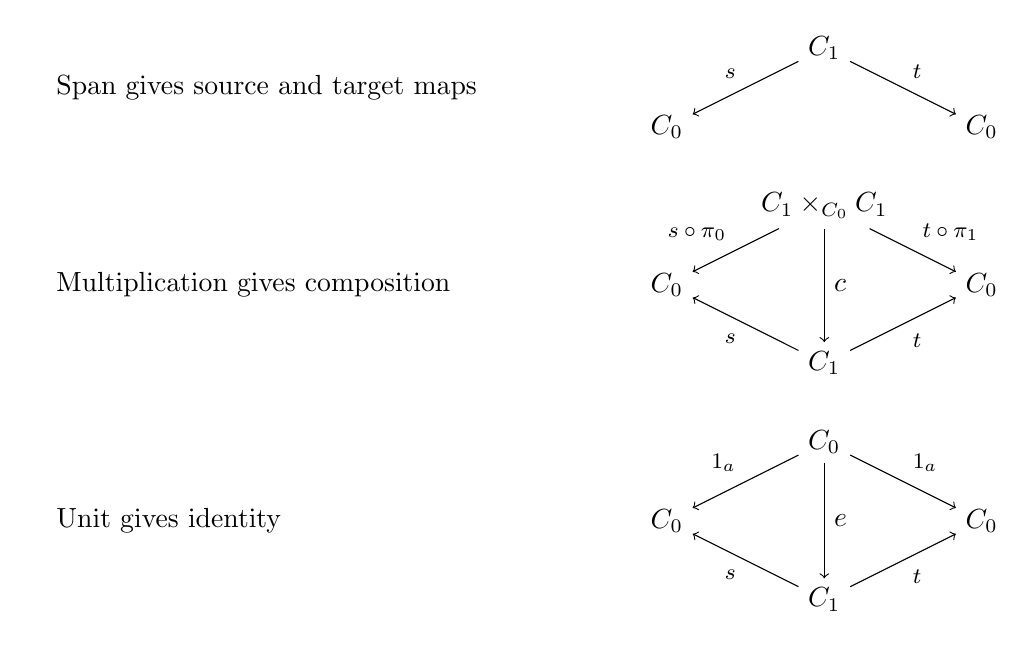
\begin{tikzpicture}
                \node[label={[align=left]right:Span gives source and target maps}] at (-10, -0.5) {};
                \node[label={[align=left]right:Multiplication gives composition}] at (-10, -3) {};
                \node[label={[align=left]right:Unit gives identity}] at (-10, -6) {};
                \node (mor) at (0, 0) {$C_1$};
                \node (ob1) at (-2, -1) {$C_0$};
                \node (ob2) at (2, -1) {$C_0$};
                \draw[->] (mor) -- node[above left]{\footnotesize$s$} (ob1);
                \draw[->] (mor) -- node[above right]{\footnotesize$t$} (ob2);
                \node (MM) at (0, -2) {$C_1\times_{C_0}C_1$};
                \node (M1) at (0, -4) {$C_1$};
                \node (O1) at (-2, -3) {$C_0$};
                \node (O2) at (2, -3) {$C_0$};
                \draw[->] (MM) -- node[above left]{\footnotesize$s\circ\pi_0$} (O1);
                \draw[->] (MM) -- node[above right]{\footnotesize$t\circ\pi_1$} (O2);
                \draw[->] (MM) -- node[right]{$c$} (M1);
                \draw[->] (M1) -- node[below left]{\footnotesize$s$} (O1);
                \draw[->] (M1) -- node[below right]{\footnotesize$t$} (O2);
                \node (O3) at (0, -5) {$C_0$};
                \node (M2) at (0, -7) {$C_1$};
                \node (O4) at (-2, -6) {$C_0$};
                \node (O5) at (2, -6) {$C_0$};
                \draw[->] (O3) -- node[above left]{\footnotesize$\mathbbm{1}_a$} (O4);
                \draw[->] (O3) -- node[above right]{\footnotesize$\mathbbm{1}_a$} (O5);
                \draw[->] (O3) -- node[right]{$e$} (M2);
                \draw[->] (M2) -- node[below left]{\footnotesize$s$} (O4);
                \draw[->] (M2) -- node[below right]{\footnotesize$t$} (O5);
            \end{tikzpicture}
            \caption{Internal category as a monad in $\mathbf{Span}(\mathcal{E})$.}
            \label{fig:internal_cat_monad}
        \end{figure}
    \end{adefinition}

    Functors between internal categories are not the only relevant morphisms. However, when defining (co)presheafs such as the hom-functor, a problem occurs. In $\mathbf{Cat}$ there exist, by definition, maps to the ambient category $\mathbf{Set}$ (ordinary category theory has a set-theoretic foundation). However, for internal categories there does not necessarily exist a morphism $\mathbf{C}\rightarrow\mathcal{E}$. To solve this problem one can consider a more general structure:
    \newdef{Internal diagram}{\index{diagram}
        A left module over a monad in $\mathbf{Span}(\mathcal{E})$. The dual notion is better known as an \textbf{internal presheaf}.
    }
    In fact, this is a specific instance of an even more general concept (for more information on the definitions and applications see \cite{maclane, johnstone}):
    \newdef{Internal profunctor}{\index{pro!functor}
        A bimodule between monads in $\mathbf{Span}(\mathcal{E})$. Together with the above definitions this gives rise to an equivalence $\mathbf{Mod}(\mathbf{Span}(\mathcal{E}))\cong\mathbf{Prof}(\mathcal{E})$.
    }

    \begin{construct}[Internal Yoneda profunctor]
        Consider an internal functor $\func{F}{A}{B}$. This functor induces two internal profunctors $\profunc{F_*}{B}{A}$ and $\profunc{F^*}{A}{B}$:
        \begin{quote}
            For $F_*$ the object span is defined as (the profunctor $F^*$ is defined similarly) \[A_0\overset{\pi_0}{\longleftarrow}A_0\times_{B_0} B_1\overset{t\circ\pi_1}{\longrightarrow}B_0.\] The action of $f\in B_1$ is given by postcomposition with $f$ in the second factor, while the action of $g\in A_1$ is given by precomposition with $Fg$ in the second factor and changing to the domain of $g$ in the first factor.
        \end{quote}
        It can easily be shown that the profunctors induced by an identity functor $\mathbbm{1}_{\mathbf{C}}$ have an object span that corresponds to the internal category $\mathbf{C}$ with the actions given by (internal) composition. In the case of $\mathcal{E}=\mathbf{Set}$ this boils down to the hom-functor. The fact that the object span is equivalent to the category $\mathbf{C}$ is essentially the Yoneda embedding. For this reason this profunctor is in general called the (internal) Yoneda profunctor $\mathcal{Y}(\mathbf{C})$.
    \end{construct}

\section{Monoidal categories}\label{section:monoidal_categories}

    \newdef{Monoidal category}{\index{monoidal!category}\index{tensor!product}\label{cat:monoidal_category}
        A category $\mathbf{C}$ equipped with a bifunctor \[-\otimes -:\mathbf{C}\times\mathbf{C}\rightarrow\mathbf{C}\] called the \textbf{tensor product} or \textbf{monoidal product}, a distinct object $\mathbf{1}$ called the \textbf{unit object}, and the following three natural isomorphisms called the \textbf{coherence maps}:
        \begin{itemize}
            \item\textbf{Associator}: $\alpha_{x,y,z}:(x\otimes y)\otimes z\cong x\otimes(y\otimes z)$;
            \item\textbf{Left unitor}: $\lambda_x:\mathbf{1}\otimes x\cong x$; and
            \item\textbf{Right unitor}: $\rho_x:x\otimes\mathbf{1}\cong x$.
        \end{itemize}
        These natural transformations are required make the \textbf{triangle} and \textbf{pentagon} diagrams \ref{fig:triangle_diagram} and \ref{fig:pentagon_diagram} commute.

        \begin{figure}[ht!]
            \centering
            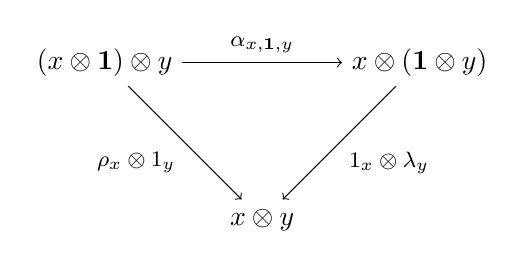
\begin{tikzpicture}
                \node (1) at (0, 0) {$(x\otimes\mathbf{1})\otimes y$};
                \node (2) at (4, 0) {$x\otimes(\mathbf{1}\otimes y)$};
                \node (3) at (2, -2) {$x\otimes y$};
                \draw[->] (1) -- node[above]{\footnotesize$\alpha_{x,\mathbf{1},y}$} (2);
                \draw[->] (1) -- node[below left]{\footnotesize$\rho_x\otimes\mathbbm{1}_y$} (3);
                \draw[->] (2) -- node[below right]{\footnotesize$\mathbbm{1}_x\otimes\lambda_y$} (3);
            \end{tikzpicture}
            \caption{Triangle diagram.}
            \label{fig:triangle_diagram}
        \end{figure}
        \begin{figure}[ht!]
            \centering
            \begin{tikzpicture}
                \node (1) at (0, 0) {$((w\otimes x)\otimes y)\otimes z$};
                \node (2) at (6, 0) {$(w\otimes(x\otimes y))\otimes z$};
                \node (3) at (-2, -3) {$(w\otimes x)\otimes(y\otimes z)$};
                \node (4) at (8, -3) {$w\otimes((x\otimes y)\otimes z)$};
                \node (5) at (3, -6) {$w\otimes(x\otimes(y\otimes z))$};
                \draw[->] (1) -- node[above]{\small$\alpha_{w,x,y}\otimes\mathbbm{1}_z$} (2);
                \draw[->] (1) -- node[above left]{\small$\alpha_{w\otimes x,y,z}$} (3);
                \draw[->] (3) -- node[below left]{\small$\alpha_{w,x,y\otimes z}$} (5);
                \draw[->] (2) -- node[above right]{\small$\alpha_{w,x\otimes y,z}$} (4);
                \draw[->] (4) -- node[below right]{\small$\mathbbm{1}_w\otimes\alpha_{x,y,z}$} (5);
            \end{tikzpicture}
            \caption{Pentagon diagram.}
            \label{fig:pentagon_diagram}
        \end{figure}
        A monoidal category for which the associator and the unitors are identity transformations is often said to be \textbf{strict}.
    }

    \begin{example}[Cartesian category]
        A monoidal category where the monoidal product is given by the ordinary product \ref{cat:product}.
    \end{example}

    \newdef{Scalar}{\index{scalar}
        In a monoidal category the scalars are defined as the endomorphisms $\mathbf{1}\rightarrow\mathbf{1}$. The set of scalars forms a commutative monoid.
    }
    \begin{property}
        Every scalar $s:\mathbf{1}\rightarrow\mathbf{1}$ induces a natural transformation $s:\mathbbm{1}_{\mathbf{C}}\Rightarrow\mathbbm{1}_{\mathbf{C}}$ with components \[s_x:x\cong\mathbf{1}\otimes x\overset{s\otimes\mathbbm{1}_x}{\longrightarrow}\mathbf{1}\otimes x\cong x.\] For every morphism $f\in\mathrm{hom}(\mathbf{C})$, the naturality square $f\circ s_x=s_y\circ f$ alo defines a morphism $s\diamond f$ that is equivalently given by $\rho_y\circ(f\otimes s)\circ\rho^{-1}_x$ (one could have used the left unitors as well). These morphisms satisfy the following well-known rules of scalar multiplication from linear algebra:
        \begin{itemize}
            \item $s\diamond(s'\diamond f) = (s\circ s')\diamond f$,
            \item $(s\diamond f)\circ(s'\diamond g) = (s\circ s')\diamond(f\circ g)$, and
            \item $(s\diamond f)\otimes(s'\diamond g) = (s\circ s')\diamond(f\otimes g)$.
        \end{itemize}
    \end{property}

    \newdef{Weak inverse}{\index{weak!inverse}
        Let $(\mathbf{C},\otimes,\mathbf{1})$ be a monoidal category and consider an object $x\in\ob{C}$. An object $y\in\ob{C}$ is called a weak inverse of $x$ if it satisfies $x\otimes y\cong\mathbf{1}$.
    }
    \remark{One can show that the existence of a one-sided weak inverse (as in the definition above) is sufficient to prove that it is in fact a two-sided weak inverse, i.e. $y\otimes x\cong\mathbf{1}$ also holds.}

    \begin{theorem}[MacLane's coherence theorem]\index{coherence!theorem}
        Consider two functors $\func{F,G}{A}{B}$ between two monoidal categories $\mathbf{A},\mathbf{B}$. Any two natural transformations $\eta,\varepsilon:F\Rightarrow G$, constructed solely from the associator and the unitors, coincide.
    \end{theorem}

\subsection{Braided categories}

    \newdef{Braided monoidal category}{\index{braiding}
        A monoidal category $(\mathbf{C},\otimes,\mathbf{1})$ equipped with a natural isomorphism \[\sigma_{x,y}:x\otimes y\cong y\otimes x\]
        that makes the two \textbf{hexagon} diagrams \ref{fig:hexagon_diagrams1} and \ref{fig:hexagon_diagrams2} commute for all $x,y,z\in\ob{C}$. The isomorphism $\sigma$ is called the \textbf{braiding} (morphism).
        \begin{figure}[ht!]
            \centering
            \begin{subfigure}[b]{0.49\textwidth}
                \centering
                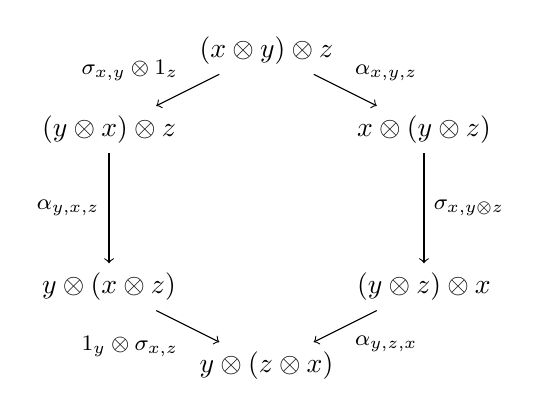
\begin{tikzpicture}
                    \node (1) at (0, 0) {$(x\otimes y)\otimes z$};
                    \node (2) at (-2, -1) {$(y\otimes x)\otimes z$};
                    \node (3) at (2, -1) {$x\otimes(y\otimes z)$};
                    \node (4) at (-2, -3) {$y\otimes(x\otimes z)$};
                    \node (5) at (2, -3) {$(y\otimes z)\otimes x$};
                    \node (6) at (0, -4) {$y\otimes(z\otimes x)$};
                    \draw[->] (1) -- node[above left]{\footnotesize$\sigma_{x,y}\otimes\mathbbm{1}_z$} (2);
                    \draw[->] (1) -- node[above right]{\footnotesize$\alpha_{x,y,z}$} (3);
                    \draw[->] (2) -- node[left]{\footnotesize$\alpha_{y,x,z}$} (4);
                    \draw[->] (3) -- node[right]{\footnotesize$\sigma_{x,y\otimes z}$} (5);
                    \draw[->] (4) -- node[below left]{\footnotesize$\mathbbm{1}_y\otimes\sigma_{x,z}$} (6);
                    \draw[->] (5) -- node[below right]{\footnotesize$\alpha_{y,z,x}$} (6);
                \end{tikzpicture}
                \caption{Hexagon diagram 1.}
                \label{fig:hexagon_diagrams1}
            \end{subfigure}
            \begin{subfigure}[b]{0.49\textwidth}
                \centering
                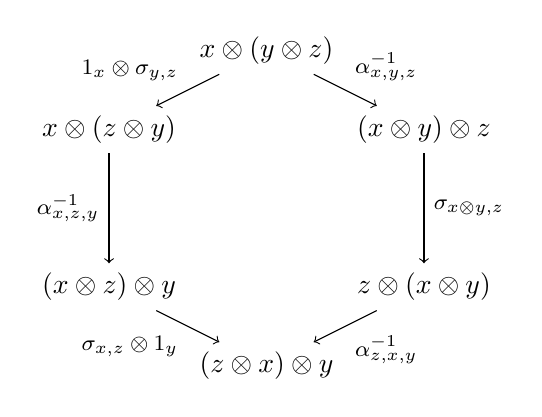
\begin{tikzpicture}
                    \node (1) at (0, 0) {$x\otimes(y\otimes z)$};
                    \node (2) at (-2, -1) {$x\otimes(z\otimes y)$};
                    \node (3) at (2, -1) {$(x\otimes y)\otimes z$};
                    \node (4) at (-2, -3) {$(x\otimes z)\otimes y$};
                    \node (5) at (2, -3) {$z\otimes(x\otimes y)$};
                    \node (6) at (0, -4) {$(z\otimes x)\otimes y$};
                    \draw[->] (1) -- node[above left]{\footnotesize$\mathbbm{1}_x\otimes\sigma_{y,z}$} (2);
                    \draw[->] (1) -- node[above right]{\footnotesize$\alpha^{-1}_{x,y,z}$} (3);
                    \draw[->] (2) -- node[left]{\footnotesize$\alpha^{-1}_{x,z,y}$} (4);
                    \draw[->] (3) -- node[right]{\footnotesize$\sigma_{x\otimes y,z}$} (5);
                    \draw[->] (4) -- node[below left]{\footnotesize$\sigma_{x,z}\otimes\mathbbm{1}_y$} (6);
                    \draw[->] (5) -- node[below right]{\footnotesize$\alpha^{-1}_{z,x,y}$} (6);
                \end{tikzpicture}
                \caption{Hexagon diagram 2.}
                \label{fig:hexagon_diagrams2}
            \end{subfigure}
            \caption{Hexagon diagram.}
            \label{fig:hexagon_diagrams}
        \end{figure}
    }
    \begin{property}[Yang-Baxter equation]\index{Yang-Baxter}
        The components $\sigma_{x,x}$ of a braiding satisfy the \textit{Yang-Baxter} equation. More generally, the braiding $\sigma$ satisfies the following equation for all objects $x,y,z\in\ob{C}$:
        \begin{gather}
            (\sigma_{y,z}\otimes\mathbbm{1}_x)\circ(\mathbbm{1}_y\otimes\sigma_{x,z})\circ(\sigma_{x,y}\otimes\mathbbm{1}_z) = (\mathbbm{1}_z\otimes\sigma_{x,y})\circ(\sigma_{x,z}\otimes\mathbbm{1}_y)\circ(\mathbbm{1}_x\otimes\sigma_{y,z}).
        \end{gather}
    \end{property}
    \remark{When drawing the above equality using string diagrams, it can be seen that the Yang-Baxter equation corresponds to the invariance of string diagrams under a \textit{Reidemeister III move}.\index{Reidemeister move}}

    \newdef{Symmetric monoidal category}{\label{cat:symmetric}
        A braided monoidal category where the braiding $\sigma$ satisfies
        \begin{gather}
            \sigma_{x,y}\circ\sigma_{y,x} = \mathbbm{1}_{x\otimes y}\,.
        \end{gather}
    }

    In Chapter \ref{chapter:hda} the theory of monoidal categories is continued.

\subsection{Monoidal functors}

    \newdef{Monoidal functor}{\index{monoidal!functor}\index{coherence!maps}
        Let $(\mathbf{A},\otimes,\mathbf{1}_{\mathbf{A}}),(\mathbf{B},\circledast,\mathbf{1}_{\mathbf{B}})$ be two monoidal categories. A functor $\func{F}{A}{B}$ is said to be monoidal if there exists:
        \begin{enumerate}
            \item A natural isomorphism $\psi_{x,y}:Fx\circledast Fy\Rightarrow F(x\otimes y)$ that makes Diagram \ref{fig:monoidal_functor1} commute.

                \begin{figure}[ht!]
                    \centering
                    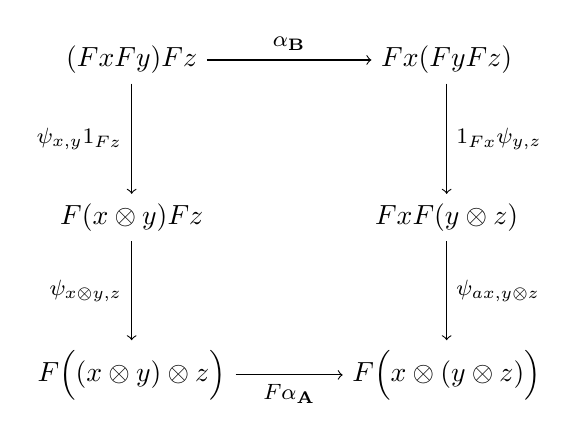
\begin{tikzpicture}
                        \node (1) at (0, 0) {$(Fx\circledast Fy)\circledast Fz$};
                        \node (2) at (4, 0) {$Fx\circledast(Fy\circledast Fz)$};
                        \node (3) at (0, -2) {$F(x\otimes y)\circledast Fz$};
                        \node (4) at (4, -2) {$Fx\circledast F(y\otimes z)$};
                        \node (5) at (0, -4) {$F\Big((x\otimes y)\otimes z\Big)$};
                        \node (6) at (4, -4) {$F\Big(x\otimes(y\otimes z)\Big)$};
                        \draw[->] (1) -- node[above]{\footnotesize$\alpha_{\mathbf{B}}$} (2);
                        \draw[->] (5) -- node[below]{\footnotesize$F\alpha_{\mathbf{A}}$} (6);
                        \draw[->] (1) -- node[left]{\footnotesize$\psi_{x,y}\circledast\mathbbm{1}_{Fz}$} (3);
                        \draw[->] (3) -- node[left]{\footnotesize$\psi_{x\otimes y,z}$} (5);
                        \draw[->] (2) -- node[right]{\footnotesize$\mathbbm{1}_{Fx}\circledast\psi_{y,z}$} (4);
                        \draw[->] (4) -- node[right]{\footnotesize$\psi_{ax,y\otimes z}$} (6);
                    \end{tikzpicture}
                    \caption{Monoidal functor.}
                    \label{fig:monoidal_functor1}
                \end{figure}
            \item An isomorphism $\phi:\mathbf{1}_{\mathbf{B}}\rightarrow F\mathbf{1}_{\mathbf{A}}$ that makes the two diagrams in Figure \ref{fig:unitality} commute.

            \begin{figure}[ht!]
                \centering
                \begin{subfigure}[b]{0.49\textwidth}
                    \centering
                    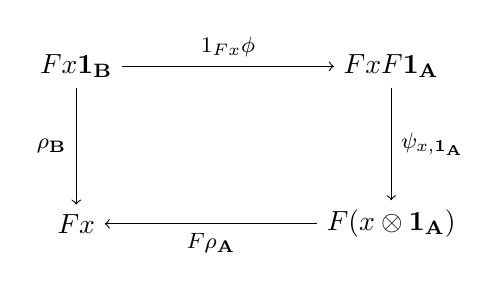
\begin{tikzpicture}
                        \node (1) at (0, 0) {$Fx\circledast\mathbf{1}_{\mathbf{B}}$};
                        \node (2) at (4, 0) {$Fx\circledast F\mathbf{1}_{\mathbf{A}}$};
                        \node (3) at (0, -2) {$Fx$};
                        \node (4) at (4, -2) {$F(x\otimes\mathbf{1}_{\mathbf{A}})$};
                        \draw[->] (1) -- node[above]{\footnotesize$\mathbbm{1}_{Fx}\circledast\phi$} (2);
                        \draw[<-] (3) -- node[below]{\footnotesize$F\rho_{\mathbf{A}}$} (4);
                        \draw[->] (1) -- node[left]{\footnotesize$\rho_{\mathbf{B}}$} (3);
                        \draw[->] (2) -- node[right]{\footnotesize$\psi_{x,\mathbf{1}_{\mathbf{A}}}$} (4);
                    \end{tikzpicture}
                \end{subfigure}
                \begin{subfigure}[b]{0.49\textwidth}
                    \centering
                    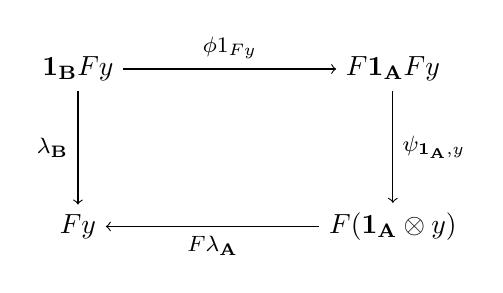
\begin{tikzpicture}
                        \node (1) at (0, 0) {$\mathbf{1}_{\mathbf{B}}\circledast Fy$};
                        \node (2) at (4, 0) {$F\mathbf{1}_{\mathbf{A}}\circledast Fy$};
                        \node (3) at (0, -2) {$Fy$};
                        \node (4) at (4, -2) {$F(\mathbf{1}_{\mathbf{A}}\otimes y)$};
                        \draw[->] (1) -- node[above]{\footnotesize$\phi\circledast\mathbbm{1}_{Fy}$} (2);
                        \draw[<-] (3) -- node[below]{\footnotesize$F\lambda_{\mathbf{A}}$} (4);
                        \draw[->] (1) -- node[left]{\footnotesize$\lambda_{\mathbf{B}}$} (3);
                        \draw[->] (2) -- node[right]{\footnotesize$\psi_{\mathbf{1}_{\mathbf{A}},y}$} (4);
                    \end{tikzpicture}
                \end{subfigure}
                \caption{Unitality diagrams.}
                \label{fig:unitality}
            \end{figure}
        \end{enumerate}
    }
    \remark{The maps $\psi$ and $\phi$ are also called \textbf{coherence maps} or \textbf{structure morphisms}.}

    \begin{property}[Canonical unit]
        For every monoidal functor $F$ there exists a canonical isomorphism $\phi:\mathbf{1}_{\mathbf{B}}\rightarrow F\mathbf{1}_{\mathbf{A}}$ defined by the commutative Diagram \ref{fig:canonical_monoidal_isom}.

        \begin{figure}[ht!]
            \centering
            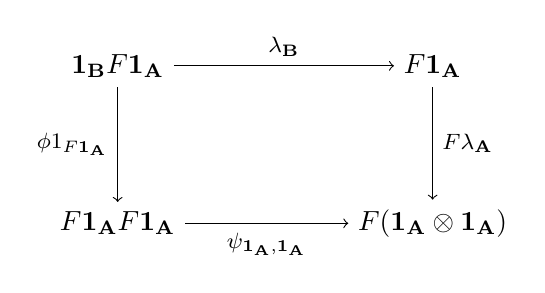
\begin{tikzpicture}
                \node (1) at (0, 0) {$\mathbf{1}_{\mathbf{B}}\circledast F\mathbf{1}_{\mathbf{A}}$};
                \node (2) at (4, 0) {$F\mathbf{1}_{\mathbf{A}}$};
                \node (3) at (0, -2) {$F\mathbf{1}_{\mathbf{A}}\circledast F\mathbf{1}_{\mathbf{A}}$};
                \node (4) at (4, -2) {$F(\mathbf{1}_{\mathbf{A}}\otimes\mathbf{1}_{\mathbf{A}})$};
                \draw[->] (1) -- node[above]{\footnotesize$\lambda_{\mathbf{B}}$} (2);
                \draw[->] (3) -- node[below]{\footnotesize$\psi_{\mathbf{1}_{\mathbf{A}}, \mathbf{1}_{\mathbf{A}}}$} (4);
                \draw[->] (1) -- node[left]{\footnotesize$\phi\circledast\mathbbm{1}_{F\mathbf{1}_{\mathbf{A}}}$} (3);
                \draw[->] (2) -- node[right]{\footnotesize$F\lambda_{\mathbf{A}}$} (4);
            \end{tikzpicture}
            \caption{Canonical unit isomorphism.}
            \label{fig:canonical_monoidal_isom}
        \end{figure}
    \end{property}

    \newdef{Lax monoidal functor}{\index{lax!monoidal functor}
        A monoidal functor for which the coherence maps are merely morphisms and not isomorphisms.
    }

    \newdef{Monoidal natural transformation}{
        A natural transformation $\eta$ between (lax) monoidal functors $(F,\psi,\phi_F)$ and $(G,\widetilde{\psi},\phi_G)$ that makes the diagrams in Figure \ref{fig:monoidal_natural_transformation} commute.
        \begin{figure}[ht!]
            \centering
            \begin{subfigure}[b]{0.49\textwidth}
                \centering
                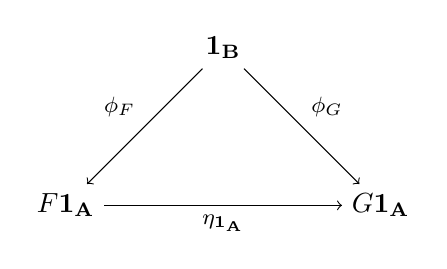
\begin{tikzpicture}
                    \node (1) at (0, 0) {$\mathbf{1}_{\mathbf{B}}$};
                    \node (2) at (-2, -2) {$F\mathbf{1}_{\mathbf{A}}$};
                    \node (3) at (2, -2) {$G\mathbf{1}_{\mathbf{A}}$};
                    \draw[->] (1) -- node[above left]{\footnotesize$\phi_F$} (2);
                    \draw[->] (1) -- node[above right]{\footnotesize$\phi_G$} (3);
                    \draw[->] (2) -- node[below]{\footnotesize$\eta_{\mathbf{1}_{\mathbf{A}}}$} (3);
                \end{tikzpicture}
            \end{subfigure}
            \begin{subfigure}[b]{0.49\textwidth}
                \centering
                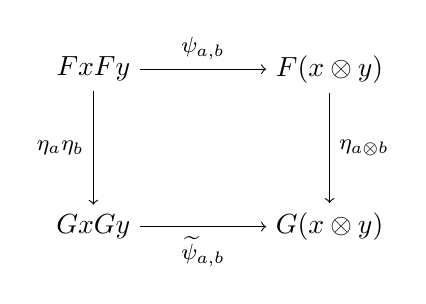
\begin{tikzpicture}
                    \node (1) at (0, 0) {$Fx\circledast Fy$};
                    \node (2) at (3, 0) {$F(x\otimes y)$};
                    \node (3) at (0, -2) {$Gx\circledast Gy$};
                    \node (4) at (3, -2) {$G(x\otimes y)$};
                    \draw[->] (1) -- node[above]{\footnotesize$\psi_{a,b}$} (2);
                    \draw[->] (3) -- node[below]{\footnotesize$\widetilde{\psi}_{a,b}$} (4);
                    \draw[->] (1) -- node[left]{\footnotesize$\eta_a\circledast\eta_b$} (3);
                    \draw[->] (2) -- node[right]{\footnotesize$\eta_{a\otimes b}$} (4);
                \end{tikzpicture}
            \end{subfigure}
            \caption{Monoidal natural transformation.}
            \label{fig:monoidal_natural_transformation}
        \end{figure}
    }

    \newdef{Monoidal equivalence}{\index{monoidal!equivalence}
        An equivalence of monoidal categories consisting of monoidal functors and monoidal natural isomorphisms.
    }
    \begin{theorem}[MacLane's strictness theorem]\index{MacLane!strictness theorem}
        Every monoidal category is monoidally equivalent to a strict monoidal category.
    \end{theorem}

\subsection{Closed categories}

    \newdef{Internal hom}{\index{internal!hom}\label{cat:internal_hom}
        Let $(\mathbf{M},\otimes,\mathbf{1})$ be a monoidal category. In this setting one can generalize the \textit{currying} procedure, i.e. the identification of maps $x\times y\rightarrow z$ with maps $x\rightarrow(y\rightarrow z)$. The internal hom-functor $\underline{\hom}$ is defined by the following natural isomorphism:
        \begin{gather}
            \hom(x\otimes y,z)\cong\hom(x,\underline{\hom}(y,z)).
        \end{gather}
        The existence of all internal homs is equivalent to the existence of a right adjoint to the tensor functor.
    }
    \begin{notation}
        The internal hom $\underline{\hom}(x,y)$ is also often denoted by $[x,y]$. From now on this convention will be followed (unless otherwise specified).
    \end{notation}
    \newdef{Closed monoidal category}{\index{closed!category}\index{Cartesian!closed}\label{cat:closed}
        A monoidal category is said to be closed monoidal if it has all internal homs. If the monoidal structure is induced by a (Cartesian) product structure, the category is often said to be \textbf{Cartesian closed}.

        A category for which all slice categories are Cartesian closed is said to be \textbf{locally Cartesian closed}. A locally Cartesian closed category with a terminal object is also Cartesian closed.
    }

    \newdef{Exponential object}{\index{exponential!object}\label{cat:exponential_object}
        In the case of Cartesian (monoidal) categories, the internal hom $\underline{\text{Hom}}(x,y)$ is called the exponential object. This object is often denoted by $y^x$.

        In Cartesian closed categories a different, but frequently used, notation is $x\Rightarrow y$. However, this notation will not be used as it might be confusion with the notation for \textit{2-morphisms}.
    }

    \newdef{Cartesian closed functor}{\index{Cartesian!closed}\label{cat:cartesian_closed_functor}
        A functor between Cartesian closed categories that preserves products and exponential objects. As such it is the natural notion of functor between Cartesian closed categories.
    }
    \begin{property}[Frobenius reciprocity]\index{Forbenius!reciprocity}
        A functor $R$ between Cartesian closed categories that admits a left adjoint $L$ is Cartesian closed if and only if the natural transformation
        \begin{gather}
            L(y\times Rx)\rightarrow Ly\times x
        \end{gather}
        is a natural isomorphism.
    \end{property}

    \begin{property}[Global elements]\label{cat:internal_hom_property}
        The following isomorphism is natural in both $x,y\in\ob{M}$:
        \begin{gather}
            \mathbf{M}(\mathbf{1},[x,y])\cong\mathbf{M}(x,y).
        \end{gather}
        It is this relation that gives the best explanation for the term ``internal hom''. One also immediately obtains the following natural isomorphism:
        \begin{gather}
            \mathbf{M}(x,[\mathbf{1},y])\cong\mathbf{M}(x,y).
        \end{gather}
        Because the Yoneda embedding is fully faithful this implies that $[\mathbf{1},y]\cong y$. Although the global elements $\mathbf{M}(\mathbf{1},y)$ do not fully specify an object $y$, this does hold internally.
    \end{property}

    \begin{property}[Symmetry]
        Let $\mathbf{M}$ be a closed monoidal category. The definition of an internal hom can also be internalized, i.e. there exists a natural isomorphism of the form
        \begin{gather}
            [x\otimes y,z]\cong[x,[y,z]].
        \end{gather}
        Furthermore, if $\mathbf{M}$ is also symmetric \ref{cat:symmetric}, there exists an internal isomorphism of the form
        \begin{gather}
            \label{cat:internal_symmetry}
            [x,[y,z]]\cong[y,[x,z]].
        \end{gather}
    \end{property}

    \newdef{Strong adjunction}{\index{adjunction!strong}
        Consider a monoidal category $\mathbf{M}$ together with two endofunctors $\func{L,R}{M}{M}$. These functors are said to form a strong adjunction if there exists a natural isomorphism
        \begin{gather}
            [Lx,y]\cong[x,Ry].
        \end{gather}
        Property \ref{cat:internal_hom_property} above implies that every strong adjunction is in particular an adjunction in the sense of Section \ref{section:adjunction}.
    }

\section{Enriched category theory}\label{section:enriched_category_theory}

    The following definition is due to \textit{B\'enabou}. It should represent the ``ideal place in which to do category theory''.
    \newdef{Cosmos}{\index{cosmos}\label{cat:cosmos}
        A complete and cocomplete closed symmetric monoidal category.
    }

    \newdef{Enriched category}{\index{category!enriched}
        Let $(\mathcal{V},\otimes,\mathbf{1})$ be a monoidal category. A $\mathcal{V}$-enriched category, also called a $\mathcal{V}$-category\footnote{Not to be confused with the notation for fibre categories \ref{cat:fibre_category}.}, consists of the following elements:
        \begin{itemize}
            \item a collection of objects $\ob{C}$, and
            \item for every pair of objects $x,y\in\ob{C}$, an object $\mathbf{C}(x,y)\in\ob{\mathcal{V}}$ for which the following morphisms exist:
            \begin{enumerate}
                \item $\text{id}_x:\mathbf{1}\rightarrow\mathbf{C}(x,x)$ giving the (enriched) identity morphism, and
                \item $\circ_{xyz}:\mathbf{C}(y,z)\otimes\mathbf{C}(x,y)\rightarrow\mathbf{C}(x,z)$ replacing the usual composition.
            \end{enumerate}
        \end{itemize}
        The associativity and unity properties are given by commutative diagrams for the $\mathrm{id}$ and $\circ$ morphisms together with the associators and unitors in $\mathcal{V}$.
    }
    \newdef{Underlying category}{
        Given a $\mathcal{V}$-enriched category $\mathbf{C}$, the underlying category $\mathbf{C}_0$ is defined as follows:
        \begin{itemize}
            \item\textbf{Objects}: $\ob{C}$
            \item\textbf{Morphisms}: $\mathcal{V}(\mathbf{1},\mathbf{C}(x,y))$,
        \end{itemize}
        where $\mathbf{1}$ is the monoidal unit in $\mathcal{V}$. This construction can be obtained as the functor $\mathcal{V}\mathbf{Cat}(\mathcal{I},-)$ where $\mathcal{I}$ is the one-object $\mathcal{V}$-category with $\mathcal{I}(\ast,\ast)\equiv\mathbf{1}$.
    }
    \begin{property}[$\mathcal{V}$ as a $\mathcal{V}$-category]
        Consider a closed monoidal category $\mathcal{V}$. This category can be given the structure $\widetilde{\mathcal{V}}$ of a $\mathcal{V}$-category by taking the hom-objects to be the internal homs, i.e. $\widetilde{\mathcal{V}}(x,y) := [x,y]$ for all $x,y\in\mathcal{V}$. Property $\ref{cat:internal_hom_property}$ then implies that there exists an isomorphism between the underlying category $\widetilde{\mathcal{V}}_0$ and the original category $\mathcal{V}$.
    \end{property}

    Given two $\mathcal{V}$-enriched categories, one can define suitable functors between them:
    \newdef{Enriched functor}{\index{functor}
        A $\mathcal{V}$-enriched functor $\func{F}{A}{B}$ consists of the following data:
        \begin{itemize}
            \item a function $F_0:\ob{A}\rightarrow\ob{B}$ (as for ordinary functors), and
            \item for every two objects $x,y\in\ob{A}$, a morphism $F_{x,y}:\mathbf{A}(x,y)\rightarrow\mathbf{B}(Fx,Fy)$ in $\mathcal{V}$.
        \end{itemize}
        These have to satisfy the ``usual'' composition and unit conditions.

        By extending Property \ref{cat:natural_end} using enriched ends, one obtains a definition of enriched natural transformations and, therefore, also a definition of enriched functor categories.:
        \begin{gather}
            \label{cat:enriched_nat_end}
            \funccat{A}{B}(F,G) := \int_{x\in\mathbf{A}}\mathbf{B}(Fx,Gx).
        \end{gather}
    }
    Given two $\mathcal{V}$-enriched functors $\func{F,G}{A}{B}$ one can also try to define $\mathcal{V}$-natural transformations by extending the usual definition of natural transformations \ref{cat:natural}:
    \newdef{Enriched natural transformation}{\index{natural!transformation}
         An ordinary natural transformation consists of an $\ob{A}$-indexed family of morphism $\eta_x:Fx\rightarrow Gx$. This can also be interpreted as an $\ob{A}$-indexed family of morphisms $\eta_x:1\rightarrow\mathbf{B}(Fx,Gx)$ from the initial object (one-element set). By analogy, a $\mathcal{V}$-natural transformation is defined as an $\ob{A}$-indexed family of morphisms $\eta_x:\mathbf{1}\rightarrow\mathbf{B}(Fx,Gx)$ from the monoidal unit. The usual naturality square is replaced by the naturality hexagon \ref{fig:v_naturality}.
    }

    The question then becomes how these two definitions are related. The end \eqref{cat:enriched_nat_end} comes equipped with a projection $\varepsilon_x:\funccat{A}{B}(F,G)\rightarrow\mathbf{B}(Fx,Gx)$. Precomposing this morphism with a morphism in the underlying category, i.e. an element of $\mathcal{V}(\mathbf{1},\funccat{A}{B}(F,G))$, exactly gives a $\mathcal{V}$-natural transformation. So the underlying category of $\funccat{A}{B}$ is the ordinary category of $\mathcal{V}$-functors and $\mathcal{V}$-natural transformations.

     \begin{figure}
        \centering
        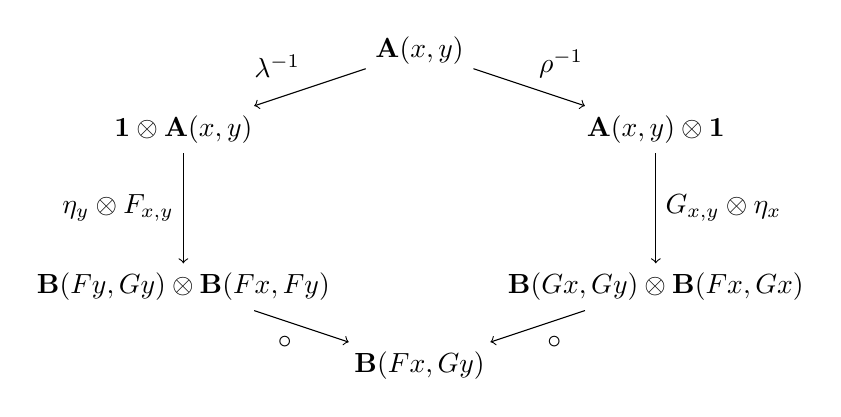
\begin{tikzpicture}
            \node (A) at (0, 0) {$\mathbf{A}(x,y)$};
            \node (IA) at (-3, -1) {$\mathbf{1}\otimes\mathbf{A}(x,y)$};
            \node (AI) at (3, -1) {$\mathbf{A}(x,y)\otimes\mathbf{1}$};
            \node (BF) at (-3, -3) {$\mathbf{B}(Fy,Gy)\otimes\mathbf{B}(Fx,Fy)$};
            \node (BG) at (3, -3) {$\mathbf{B}(Gx,Gy)\otimes\mathbf{B}(Fx,Gx)$};
            \node (B) at (0, -4) {$\mathbf{B}(Fx,Gy)$};
            \draw[->] (A) -- node[above left]{$\lambda^{-1}$} (IA);
            \draw[->] (A) -- node[above right]{$\rho^{-1}$} (AI);
            \draw[->] (IA) -- node[left]{$\eta_y\otimes F_{x,y}$} (BF);
            \draw[->] (AI) -- node[right]{$G_{x,y}\otimes\eta_x$} (BG);
            \draw[->] (BF) -- node[below left]{$\circ$} (B);
            \draw[->] (BG) -- node[below right]{$\circ$} (B);
        \end{tikzpicture}
        \caption{$\mathcal{V}$-naturality diagram.}
        \label{fig:v_naturality}
     \end{figure}

\subsection{Enriched constructions}

    \newdef{Functor tensor product}{\index{tensor!product}\label{cat:functor_tensor_product}
        Consider a covariant functor $\func{G}{C}{\mathcal{V}}$ and a contravariant functor $\cfunc{F}{C}{\mathcal{V}}$ into a monoidal category $\mathcal{V}$, where $\mathbf{C}$ does not have to be enriched over $\mathcal{V}$. The tensor product of $F$ and $G$ is defined as the following coend:
        \begin{gather}
            F\otimes_{\mathbf{C}}G := \int^{x\in\mathbf{C}}Fx\otimes Gx.
        \end{gather}
    }
    It should be noted that the above tensor product does not produce a new functor, instead it only gives an object in $\mathcal{V}$. A different type of tensor product, one that does give a functor, exists in the enriched setting (note that there is no relation between these two definitions):
    \newdef{Day convolution}{\index{Day convolution}
        Consider a monoidally cocomplete category $\mathcal{V}$, i.e. cocomplete monoidal category for which the tensor product bifunctor is cocontinuous in each argument, together with a $\mathcal{V}$-enriched category $\mathbf{C}$. The convolution or tensor product (if it exists) of two $\mathcal{V}$-enriched functors $\func{F,G}{C}{\mathcal{V}}$ is defined as the following coend:
        \begin{gather}
            F\otimes_{\text{Day}}G := \iint^{x,y\in\mathbf{C}}\mathbf{C}(x\otimes y,-)\otimes Fx\otimes Gy.
        \end{gather}
    }
    \begin{property}[Monoidal structure]
        In the case where $\mathbf{M}$ is a closed symmetric monoidal category, the Day convolution is associative and, hence, defines a monoidal structure on the functor category $[\mathbf{C},\mathbf{M}]$. The tensor unit is given by the functor (co)represented by the tensor unit in $\mathbf{C}$.
    \end{property}

    \newdef{Copower}{\index{co-!power}\index{power} % Both terms are indexed since copowers are rather important on their own.
        Consider a $\mathcal{V}$-enriched category $\mathbf{C}$. The copower (or tensor) functor $\func{\cdot}{\mathcal{V}\times C}{C}$ is defined by the following natural isomorphism:
        \begin{gather}
            \mathbf{C}(v\cdot x,y)\cong[v,\mathbf{C}(x,y)],
        \end{gather}
        where the bracket $[-,-]$ on the right-hand side denotes the internal hom in $\mathcal{V}$. Dually, the power (or cotensor) functor $\func{[-,-]}{\mathcal{V}\times C}{C}$ is defined by the following natural isomorphism:
        \begin{gather}
            \mathbf{C}(x,[v,y])\cong[v,\mathbf{C}(x,y)],
        \end{gather}
        where the bracket $[-,-]$ on the right-hand side again denotes the internal hom in $\mathcal{V}$. If an enriched category admits all (co)powers, it is said to be \textbf{(co)powered} (over its enriching category).
    }
    \remark{Equation \eqref{cat:internal_symmetry} says that every (closed) symmetric monoidal category $\mathbf{M}$ is powered over itself, the power just being the internal hom. The same holds for the copower, which is just the usual tensor product functor.}

    \begin{example}[Disjoint unions]
        Every (co)complete (locally) small category $\mathbf{C}$ admits the structure of a $\mathbf{Set}$-(co)powered category:
        \begin{gather}
            x^S := \prod_{s\in S}x\\
            S\cdot x := \bigsqcup_{s\in S}x.
        \end{gather}
    \end{example}

    The definition and properties of internal hom-functors and (co)powers can be formalized as follows:
    \newdef{Two-variable adjunction}{\index{adjunction}\label{cat:two_variable_adjunction}
        Consider three categories $\mathbf{A,B}$ and $\mathbf{C}$. A two-variable adjunction $\mathbf{A}\times\mathbf{B}\rightarrow\mathbf{C}$ consists of three bifunctors:
        \begin{itemize}
            \item $\func{-\otimes-}{A\times B}{C}$,
            \item $\mathrm{hom}_L:\mathbf{A}^{op}\times\mathbf{C}\rightarrow\mathbf{B}$, and
            \item $\mathrm{hom}_R:\mathbf{B}^{op}\times\mathbf{C}\rightarrow\mathbf{A}$
        \end{itemize}
        admitting the following natural isomorphisms:
        \begin{gather}
            \mathbf{C}(x\otimes y,z)\cong\mathbf{A}(x,\mathrm{hom}_R(y,z))\cong\mathbf{B}(y,\mathrm{hom}_L(x,z)).
        \end{gather}
        It should be noted that fixing any of the variables gives rise to ordinary adjunctions in the sense of Section \ref{section:adjunction}.
    }
    \begin{property}[Powers and copowers]
        A category $\mathbf{C}$ enriched over a monoidal category $\mathcal{V}$ is powered and copowered over $\mathcal{V}$ exactly if the hom-functor $\mathbf{C}^{op}\times\mathbf{C}\rightarrow\mathcal{V}$ is the right adjoint in an enriched two-variable adjunction. The power and copower functors are then given by the other two adjoints.
    \end{property}

    The following definition constructs Kan extensions in the enriched setting (these can be shown to reduce to \ref{cat:kan_extension} when enriching over $\mathbf{Set}$):
    \newadef{Kan extension}{\index{Kan!extension}\label{cat:enriched_kan_extension}
        Let $\mathbf{A,B}$ and $\mathbf{C}$ be categories enriched over a monoidal category $\mathcal{V}$. If $\mathbf{B}$ is assumed to be copowered over $\mathcal{V}$, one can define the left Kan extension of $\func{F}{A}{B}$ along $\func{G}{A}{C}$ as a coend:
        \begin{gather}
            \text{Lan}_GF := \int^{x\in\mathbf{A}}\mathbf{C}(Gx,-)\cdot Fx.
        \end{gather}
        If $\mathbf{B}$ is assumed to be powered over $\mathcal{V}$, one can define the right Kan extension as an end:
        \begin{gather}
            \text{Ran}_GF := \int_{x\in\mathbf{A}}[\mathbf{C}(-,Gx),Fx].
        \end{gather}
    }
    \remark{By choosing $\mathcal{V}=\mathbf{Set},\mathbf{C}=\mathbf{A}$ and $G=\mathbbm{1}_{\mathbf{A}}$ in the previous definition, one obtains the ninja Yoneda lemma \ref{cat:ninja_yoneda}.}
    \begin{property}
        Kan extensions computed using (co)ends as above are pointwise in the sense of Definition \ref{cat:preservation_kan_extension}.
    \end{property}

    \newadef{Functor tensor product}{\index{tensor!product}
        Let $\mathbf{B}$ be a $\mathcal{V}$-enriched category. Consider a covariant functor $\func{G}{A}{B}$ and a contravariant functor $\cfunc{F}{A}{\mathcal{V}}$. The tensor product \ref{cat:functor_tensor_product} can be generalized whenever $\mathbf{B}$ is copowered over $\mathcal{V}$:
        \begin{gather}
            \label{cat:copower_product}
            F\otimes_{\mathbf{A}}G := \int^{x\in\mathbf{A}}Fx\cdot Gx.
        \end{gather}
    }

\subsection{Weighted (co)limits}\index{limit!weighted}

    In this section the definition of ordinary limits and, in particular, the defining universal property \ref{cat:limit_uproperty} is revisited. In this construction the constant functor $\Delta_x$ was one of the main ingredients. This functor can be factorized as $\mathbf{I}\rightarrow1\rightarrow\mathbf{C}$, where $1$ denotes the terminal category. On the level of morphisms this factorization takes the form $\mathbf{I}(i,j)\rightarrow\ast\rightarrow\mathbf{C}(x,x)$, where $\ast$ denotes the terminal one-element set. However, whenever the enriching context is not $\mathbf{Set}$, one does not necessarily have access to a terminal object.

    To avoid this issue, limits will first be redefined as representing objects. To this end, consider a general diagram $\func{D}{I}{C}$. By postcomposition with the Yoneda embedding one obtains the presheaf-valued diagram $\mathbf{C}(-,D-):\mathbf{I}\rightarrow[\mathbf{C}^{op}, \mathbf{Set}]$. Since presheaf categories are complete (Example \ref{cat:complete_presheaf_category}), the limit of this diagram exists: \[\mathbf{Set}(S,\lim\mathbf{C}(x,D-))\cong\funccat{I}{Set}(\Delta_S, \mathbf{C}(x,D-)).\] By restricting to the terminal set $S=\ast$, one obtains \[\lim\mathbf{C}(x,D-)\cong\funccat{I}{Set}(\Delta_\ast, \mathbf{C}(x,D-)).\] If this presheaf is representable, one can use the continuity of the hom-functor, together with the fact that the Yoneda embedding is fully faithful, to show that the representing object is (isomorphic to) $\lim D$, i.e.
    \begin{gather}
        \funccat{I}{Set}(\Delta_\ast,\mathbf{C}(x,D-))\cong\mathbf{C}(x,\lim D).
    \end{gather}

    ?? CLEAN THIS UP (note that continuity and pointwise definition was already mentioned for ordinary limits) ??

    \newdef{Weighted limit}{\index{limit!conical}\label{cat:weighted_limit}
        This definition can now be generalized by replacing the constant functor $\Delta_\ast$ by any functor $\func{W}{I}{Set}$. A representing object is then called the $W$-weighted limit of $D$. This object is often denoted by $\wlim{W}D$ or $\{W,D\}$. To distinguish weighted limits from ordinary ones, the latter are sometimes called \textbf{conical limits}.
    }

    \begin{remark}
        A motivation for this construction is the following. As was already pointed out in Remark \ref{cat:global_elements_remark}, the mere knowledge of global elements $1\rightarrow x$ is often not enough to characterize an object $x$. In general one should look at the collection of generalized elements. When applying this ideology to the case of cones, one sees that replacing the functor $\Delta_\ast$ by a more general functor is the same as replacing the global elements $\ast\rightarrow Di$ by generalized elements $Wi\rightarrow Di$.
    \end{remark}

    The generalization to the enriched setting is now evident. There is no reference to the terminal object left, so one can replace $\mathbf{Set}$ by any enriching category. In the enriched setting, (co)end formulas for (weighted) limits will often be used:
    \newformula{Enriched weighted limits}{\label{cat:weighted_limits}
        By expressing the natural transformations as an end as in Equation \eqref{cat:natural_end} and by using the canonical powering in $\mathbf{Set}$, one can express ordinary weighted limits as follows:
        \begin{gather}
            \wlim{W}D\cong\int_{i\in\mathbf{I}}[Wi,Di].
        \end{gather}
        The generalization to other enriching categories is now straightforward. Consider a diagram $\func{D}{I}{C}$ and a weight functor $\func{W}{I}{\mathcal{V}}$, where $\mathbf{C}$ is $\mathcal{V}$-enriched. If $\mathbf{C}$ is powered over $\mathcal{V}$, the $W$-weighted limit of $D$ is defined by the same formula as above:
        \begin{gather}
            \wlim{W}D:=\int_{i\in I}[Wi,Di].
        \end{gather}
        In a similar way one can define weighted colimits in copowered $\mathcal{V}$-categories as coends:
        \begin{gather}
            \colim^WD:=\int^{i\in I}Wi\cdot Di.
        \end{gather}
        Here the weight functor $W$ is required to be contravariant since colimits (and cocones in general) are natural transformations between contravariant functors.
    }
    \begin{property}[Weighted limits are Hom-objects]
        In the case $\mathbf{C}=\mathcal{V}$, the powering functor becomes the internal hom and, therefore, one sees that weighted limits are given by (enriched) natural transformations (as was the case for ordinary conical limits).
    \end{property}

    In the following example the weighted colimit is calculated with respect to the Yoneda embedding:
    \begin{example}[Hom-functor]
        Consider a diagram $\func{D}{I}{C}$. When using the Yoneda embedding $\mathcal{Y}i = \mathbf{I}(-,i)$ as the weight functor, one obtains the following property by virtue of the Yoneda lemma:
        \begin{gather}
            \label{cat:weighted_hom_colimit}
            \colim^{\mathcal{Y}i}D\cong Di.
        \end{gather}
        A similar statement for weighted limits can be obtained with the covariant Yoneda embedding.
    \end{example}
    \newadef{Weighted (co)limits}{
        The above property can be used to axiomatize small weighted (co)limits in bicomplete categories:
        \begin{enumerate}
            \item\textbf{Yoneda}: For every object $i\in\ob{I}$ there exist isomorphisms
            \begin{gather}
                \wlim{\mathbf{I}(i,-)}D\cong Di\qquad\text{and}\qquad\colim^{\mathbf{I}(-,i)}D\cong Di.
            \end{gather}
            \item\textbf{Cocontinuity}: The weighted (co)limit functors are cocontinuous in the weights.
        \end{enumerate}
    }

    One can also express Kan extensions as weighted limits:
    \begin{property}[Kan extensions]\index{Kan!extension}
        Consider functors $\func{F}{A}{B}$ and $\func{G}{A}{C}$. If for every $x\in\ob{C}$ the weighted limit $\wlim{\mathbf{C}(x,G-)}F$ exists, these limits can be combined into a functor that can be shown to be the right Kan extension $\text{Ran}_GF$. The left Kan extension can be obtained as a weighted colimit.
    \end{property}

\section{Abelian categories}\label{section:abelian_categories}
\subsection{Additive and Abelian categories}

    \newdef{Pre-additive category}{
        A (locally small) category enriched over $\mathbf{Ab}$, i.e. a category in which every hom-set is an Abelian group and composition is bilinear.
    }

    \begin{property}\index{zero!object}
        Let $\mathbf{A}$ be a pre-additive category. The following statements are equivalent for an object $x\in\ob{A}$:
        \begin{itemize}
            \item $x$ is initial,
            \item $x$ is final, or
            \item $\mathbbm{1}_x = 0$.
        \end{itemize}
        It follows that every initial/terminal object in a pre-additive category is automatically a zero object \ref{cat:zero_object}.
    \end{property}
    \begin{property}[Biproducts]\index{biproduct}\index{direct!sum}
        In a pre-additive category the following isomorphism holds for all finitely indexed sets $\{x_i\}_{i\in I}$:
        \begin{gather}
            \prod_{i\in I}x_i\cong\bigsqcup_{i\in I}x_i.
        \end{gather}
        Finite (co)products in pre-additive categories are often called \textbf{direct sums}. In general, if a product and coproduct exist and are equal, one also speaks of a \textbf{biproduct}.
    \end{property}

    \newdef{Additive category}{\index{additive!category}
        A pre-additive category in which all finite products exist.
    }

    When working with additive categories, it is generally assumed that the associated functors are of a specific type:
    \newdef{Additive functor}{\index{additive!functor}\label{cat:additive_functor}
        Let $\mathbf{A},\mathbf{A'}$ be additive categories. A functor $\func{F}{A}{A'}$ is said to be additive if it preserves finite biproducts:
        \begin{enumerate}
            \item It preserves zero objects: $F\,0_{\mathbf{A}}\cong0_{\mathbf{A}'}$.
            \item There exists a natural isomorphism $F(x\oplus y)\cong Fx\oplus Fy$.
        \end{enumerate}
        This notion can be generalized to pre-additive categories. A functor between pre-additive categories is said to be additive if it acts as a group morphism on hom-spaces.
    }

    \newdef{Grothendieck group}{\index{Grothendieck!group}
        Let $\mathbf{A}$ be an additive category and consider its decategorification \ref{cat:decategorification}. This set carries the structure of an Abelian monoid and, hence, the Grothendieck construction \ref{group:grothendieck_completion} can be applied to obtain an Abelian group $K(\mathbf{A})$. This group is called the Grothendieck group of $\mathbf{A}$.
    }

    In a (pre-)additive category one can some classical notions from (homological) algebra such as images and kernels:
    \newdef{Kernel}{\index{kernel}
        Let $f:x\rightarrow y$ be a morphism. A\footnote{Note the word ``\textit{a}''. The kernel of a morphism is only determined up to an isomorphism.} kernel of $f$ is a morphism $k:z\rightarrow x$ such that:
        \begin{enumerate}
            \item $f\circ k = 0$.
            \item\textbf{Universal property}: Every morphism $k':z'\rightarrow x$ such that $f\circ k' = 0$ factors uniquely through $k$.
        \end{enumerate}
        This implies that a kernel of $f$ could equivalently be defined as the equalizer of $f$ and $0$.
    }
    \begin{notation}[Kernel]
        If the kernel of $f:x\rightarrow y$ exists, it is denoted by $\ker(f)$.
    \end{notation}

    \newdef{Cokernel}{
        Let $f:x\rightarrow y$ be a morphism. A cokernel of $f$ is a morphism $p:y\rightarrow z$ such that:
        \begin{enumerate}
            \item $p\circ f = 0$.
            \item\textbf{Universal property}: Every morphism $p':y\rightarrow z'$ such that $p'\circ f = 0$ factors uniquely through $p$.
        \end{enumerate}
        This implies that a cokernel of $f$ could equivalently be defined as the coequalizer of $f$ and 0.
    }
    \begin{notation}[Cokernel]
        If the cokernel of $f:x\rightarrow y$ exists, it is denoted by $\text{coker}(f)$.
    \end{notation}
    \begin{remark}
        The name and notation of the kernel and the cokernel (in the categorical sense) is explained by remarking that $\ker(f)$ represents the functor \[F:z\mapsto\ker\Big(\mathbf{C}(z, x)\rightarrow\mathbf{C}(z,y)\Big),\] where $\ker$ denotes the algebraic kernel \ref{group:kernel}, and similarly for he cokernel.
    \end{remark}

    \newdef{Pseudo-Abelian category}{\label{cat:pseudo_abelian}
        An additive category in which every projection/idempotent has a kernel.
    }
    \newdef{Pre-Abelian category}{
        An additive category in which every morphism has a kernel and cokernel.
    }
    \newdef{Abelian category}{\index{Abelian!category}
        A pre-Abelian category in which every mono is a kernel and every epi is a cokernel or, equivalently, if for every morphism $f$ there exists an isomorphism
        \begin{gather}
            \text{coker}(\ker(f))\cong\ker(\text{coker}(f)).
        \end{gather}
    }

    \begin{property}[Injectivity and surjectivity]
        In Abelian categories a morphism is monic if and only if it is injective, i.e. its kernel is 0. Analogously, a morphism is epic if and only if it is surjective, i.e. its cokernel is 0.
    \end{property}

    \begin{example}[$k$-linear category]\index{category!linear}
        Let $\mathbf{Vect}_k$ denote the category of vector spaces over the base field $k$. A $k$-linear category is a category enriched over $\mathbf{Vect}_k$. (If the base field is clear, the subscript is often left implicit.)
    \end{example}

\subsection{Exact functors}

    \newdef{Exact functor}{\index{exact!functor}
        Let $\func{F}{A}{A'}$ be an additive functor between additive categories.
        \begin{itemize}
            \item $F$ is said to be left-exact if it preserves kernels.
            \item $F$ is said to be right-exact if it preserves cokernels.
            \item $F$ is said to be exact if it is both left- and right-exact.
        \end{itemize}
    }
    \begin{result}
        The previous definition implies the following properties (which can in fact be used as an alternative definition):
        \begin{itemize}
            \item If $F$ is left-exact, it maps an exact sequence of the form \[0\longrightarrow x\longrightarrow y\longrightarrow z\]
            to an exact sequence of the form \[0\longrightarrow Fx\longrightarrow Fy\longrightarrow Fz.\]
            \item If $F$ is right-exact, it maps an exact sequence of the form \[x\longrightarrow y\longrightarrow z\longrightarrow 0\]
            to an exact sequence of the form \[Fx\longrightarrow Fy\longrightarrow Fz\longrightarrow 0.\]
            \item If $F$ is exact, it maps short exact sequences to short exact sequences.
        \end{itemize}
    \end{result}

    \begin{notation}[Left or right]
        The category of left modules ${}_R\mathbf{Mod}$ over a ring $R$ is equivalent (as an Abelian category) to the category of right modules $\mathbf{Mod}_{R^{op}}$ over the opposite ring $R$. For this reason one often makes no difference between left and right modules (only bimodules are truly relevant) and ``the category of $R$-modules'' is just denoted by $R\mathbf{Mod}$.
    \end{notation}

    \begin{theorem}[Freyd-Mitchell embedding theorem]\index{Freyd-Mitchell}\index{embedding!theorem|see{Freyd-Mitchell}}\label{cat:freyd_mitchell}
        Every small Abelian category admits a fully faithful, exact functor into a category of the form $R\mathbf{Mod}$ for some unital ring $R$.
    \end{theorem}

    \begin{theorem}[Eilenberg-Watts]\index{Eilenberg-Watts}
        Let $R,S$ be two (not necessarily unital) rings. The tensor product functor induces an equivalence between the category of $R\text{-}S$-bimodules and the category of cocontinuous functors $R\mathbf{Mod}\rightarrow S\mathbf{Mod}$.
    \end{theorem}

\subsection{Finiteness}

    \newdef{Simple object}{\index{simple!object}
        Let $\mathbf{A}$ be an Abelian category. An object $a\in\ob{A}$ is said to be simple if the only subobjects of $a$ are $0$ and $a$ itself. An object is said to be semisimple if it is a direct sum of simple obejcts.
    }
    \newdef{Semisimple category}{
        A category is said to be semisimple if every object is semisimple (where in general the direct sums are taken over finite index sets).
    }

    \newdef{Jordan-H\"older series}{\index{finite}
        A filtration \[0\longrightarrow x_1\longrightarrow x_2\longrightarrow\cdots\longrightarrow x_n=x\] of an object $x$ is said to be a Jordan-H\"older series if the quotient objects $x_i/x_{i-1}$ are simple for all $i\leq n$. If the series has finite length, the object $x$ is said to be \textbf{finite}.
    }
    \begin{theorem}[Jordan-H\"older]\index{Jordan-H\"older}
        If an object in an Abelian category is finite, all of its Jordan-H\"older series have the same length. In particular, the multiplicities of simple objects are the same for all such series.
    \end{theorem}

    \begin{theorem}[Krull-Schmidt]\index{Krull-Schmidt}\index{indecomposable}
        Any object in an Abelian category of finite length admits a unique decomposition as a direct sum of indecomposable objects\footnote{An object is \textbf{indecomposable} if it cannot be written as a direct sum of its subobjects.}.
    \end{theorem}

    \newdef{Locally finite}{\label{cat:locally_finite}
        A $k$-linear Abelian category is said to be locally finite if it satisfies the following conditions:
        \begin{enumerate}
            \item every hom-space is finite-dimensional, and
            \item every object has finite length.
        \end{enumerate}
    }
    \newdef{Finite}{\index{finite}
        A $k$-linear Abelian category is said to be finite if it satisfies the following conditions:
        \begin{enumerate}
            \item It is locally finite.
            \item It has enough projectives or, equivalently, every simple object has a \textit{projective cover}.
            \item The set of isomorphism classes of simple objects is finite.
        \end{enumerate}
    }

    \begin{theorem}[Schur's lemma]\index{Schur's lemma}\label{cat:schur_lemma}
        Let $\mathbf{A}$ be an Abelian category. For every two simple objects $x,y$, all nonzero morphisms $x\rightarrow y$ are isomorphisms. In particular, if $x,y$ are two non-isomorphic simple objects, then $\mathbf{A}(x,y)=0$. Furthermore, $\mathbf{A}(x,x)$ is a division ring for every simple object $x$.
    \end{theorem}
    \begin{result}
        If $\mathbf{A}$ is locally finite and $k$ is algebraically closed, then $\mathbf{A}(x,x)\cong k$ for all simple objects $x$. This follows from the fact that the only finite-dimensional division algebra over an algebraically closed field is the field itself.
    \end{result}

    The Freyd-Mitchell theorem \ref{cat:freyd_mitchell} can be adapted to the finite linear case as follows:
    \begin{theorem}[Deligne]\index{Deligne}
        Every finite $k$-linear Abelian category is $k$-linearly equivalent to a category of the form $A\mathbf{Mod}^{\text{\emph{fin}}}$ for $A$ a finite-dimensional $k$-algebra.
    \end{theorem}

    \begin{construct}[Deligne tensor product]\index{Deligne!tensor product}\index{tensor!product}
        Let $\mathbf{A},\mathbf{B}$ be two Abelian categories. Their Deligne (tensor) product is defined (if it exists) as the category $\mathbf{A}\boxtimes\mathbf{B}$ for which there exists a bijection between right exact functors $\mathbf{A}\boxtimes\mathbf{B}\rightarrow\mathbf{C}$ and right exact functors $\mathbf{A}\times\mathbf{B}\rightarrow\mathbf{C}$ (the latter being right exact in each argument).

        For finite Abelian categories it can be shown that their Deligne product always exists. By the Deligne embedding theorem one can find an explicit description. Consider two finite-dimensional $k$-algebras $A, B$. The category $A\mathbf{Mod}^{\text{fin}}\boxtimes B\mathbf{Mod}^{\text{fin}}$ is equivalent to the category $A\otimes_kB\mathbf{Mod}^{\text{fin}}$.
    \end{construct}

\section{\difficult{Higher category theory}}\label{cat:higher_category_theory}
\subsection{\texorpdfstring{$n$-categories}{n-categories}}

    \newdef{$n$-category}{\index{n-category}
        A (strict) $n$-category consists of:
        \begin{itemize}
            \item objects (0-morphisms),
            \item 1-morphisms going between 0-morphisms,
            \item ...
            \item $n$-morphisms going between $(n-1)$-morphisms,
        \end{itemize}
        such that the composition of $k$-morphisms ($k\leq n$) is associative and satisfies the unit laws as required in an ordinary category. By generalizing this definition to arbitrary $n$ one can define the notion of a (strict) $\infty$-category.

        If one relaxes the associativity and unit laws up to higher coherent morphisms, one obtains the notion a weak $n$-category. Explicit definitions for such categories have been constructed up to tetracategories $(n=4)$. However, this construction by \textit{Trimble} takes about 50 pages of diagrams.
    }
    \sremark{$n$-morphisms are also called \textbf{$n$-cells}. This makes their relation to topological spaces (and in particular simplicial spaces) more visible.}

    \begin{example}
        The classical examples of a 1-category and 2-category are $\mathbf{Set}$ and $\mathbf{Cat}$, respectively.
    \end{example}

    \begin{property}[Composition in 2-categories]\index{interchange law}
        2-morphisms can be composed in two different ways:
        \begin{itemize}
            \item\textbf{Horizontal composition}:
                Consider two 2-morphisms $\alpha:f\Rightarrow g$ and $\beta:f'\Rightarrow g'$ where $f'\circ f$ and $g'\circ g$ are well-defined. These 2-morphisms can be composed as \[\beta\circ\alpha: f'\circ f\Rightarrow g'\circ g.\]
            \item\textbf{Vertical composition}:
                Consider two 2-morphisms $\alpha:f\Rightarrow g$ and $\beta:g\Rightarrow h$ where $f,g$ and $h$ have the same domain and codomain. These 2-morphisms can be composed as \[\beta\cdot\alpha:f\Rightarrow h.\]
        \end{itemize}
        As a consistency condition the horizontal and vertical composition are required to satisfy the following \textbf{interchange law}:
        \begin{gather}
            (\alpha\cdot\beta)\circ(\gamma\cdot\delta) = (\alpha\circ\gamma)\cdot(\beta\circ\delta).
        \end{gather}
    \end{property}
    \newdef{\texorpdfstring{$(n,r)$-category}{(n,r)-Category}}{
        A higher ($\infty$-)category for which
        \begin{itemize}
            \item all parallel $k$-morphisms with $k>n$ are equivalent and, hence, trivial.
            \item all $k$-morphisms with $k>r$ are invertible (or equivalences in the fully weak $\infty$-sense).
        \end{itemize}
    }

    \newdef{Weak inverse}{\index{weak!inverse}
        Let $\mathbf{C}$ be a 2-category. A 1-morphism $f:x\rightarrow y$ is weakly invertible if there exist a 1-morphism $g:y\rightarrow x$ and 2-isomorphisms $g\circ f\Rightarrow\mathbbm{1}_x$ and $f\circ g\Rightarrow\mathbbm{1}_y$.
    }

    At this point it should be obvious that the definition of a unit-counit adjunction \ref{cat:unit_counit_adjunction} can be generalized to general 2-categories:
    \newdef{Adjunction in 2-category}{
        Let $\mathbf{C}$ be a 2-category. An adjunction in $\mathbf{C}$ is a pair of 1-morphisms $F:x\rightarrow y$ and $G:y\rightarrow x$ together with 2-morphisms $\varepsilon:F\circ G\Rightarrow\mathbbm{1}_y$ and $\eta:\mathbbm{1}_x\Rightarrow G\circ F$ that satisfy the zig-zag identities.
    }
    \begin{remark}[Duals and adjunctions]
        By looking at the defining relations of duals in a rigid monoidal category (Section \ref{section:duality} further on), it should be clear that these are in fact the same as the defining relations of the unit and counit of an adjunction. This is a consequence of the fact that a 2-category with a single object can be regarded as a (strict) monoidal category where the composition in the 2-category becomes the tensor product in the monoidal category. Similarly, adjoint 1-morphisms in the 2-category become duals in the monoidal category.
    \end{remark}

    \begin{property}[Monoidal categories]\index{monoidal!category}\index{delooping!of monoidal categories}\label{cat:monoidal_or_2}
        Consider a monoidal category $(\mathbf{C},\otimes,\mathbf{1})$. From this monoidal category one can construct the so-called \textbf{delooping} bicategory $\mathbf{BC}$ in the following way:
        \begin{itemize}
            \item There is a single object $\ast$.
            \item The 1-morphisms in $\mathbf{BC}$ are the objects in $\mathbf{C}$.
            \item The 2-morphisms in $\mathbf{BC}$ are the morphisms in $\mathbf{C}$.
            \item Horizontal composition in $\mathbf{BC}$ is the tensor product in $\mathbf{C}$.
            \item Vertical composition in $\mathbf{BC}$ is composition in $\mathbf{C}$.
        \end{itemize}
        Conversely, every 2-category with a single object comes from a monoidal category. Hence, the 2-category of (pointed) 2-categories with a single object and the 2-category of monoidal categories are equivalent. (This property and its generalizations are the content of the \textit{delooping hypothesis}.)

        In the same way one can deloop a braided monoidal category twice and find an identification with a one-object tricategory with one 1-morphism. However, this identification is not a trivial one as it makes use of the Eckmann-Hilton argument to identify different monoidal structures on this tricategory. (See also Section \ref{section:monoidal_n_cat}.)
    \end{property}

\subsection{\texorpdfstring{$n$-functors}{n-functors}}

    \newdef{2-functor}{\index{pseudo!functor}\label{cat:pseudofunctor}
        A 2-functor $\func{F}{A}{B}$ (often called a \textbf{pseudofunctor}) is a morphism between bicategories. It consists of the following data:
        \begin{itemize}
            \item a function $F_0:\ob{A}\rightarrow\ob{B}$, and
            \item for every two objects $x,y\in\ob{A}$, a functor $F_{x,y}:\mathbf{A}(x,y)\rightarrow\mathbf{B}(Fx,Fy)$.
        \end{itemize}
        The function $F_0$ and the functors $F_{x,y}$ are also often denoted by $F$ by abuse of notation. This data is required to satisfy some coherence conditions. These are specified by the following data:
        \begin{enumerate}
            \item\textbf{Associator}: For every pair of composable 1-morphisms $f\circ g$ in $\mathrm{hom}(\mathbf{A})$, a 2-isomorphism $\gamma_{f,g}:Ff\circ Fg\Rightarrow F(f\circ g)$ such that for every triple of composable morphisms $f\circ g\circ h$ in $\mathrm{hom}(\mathbf{A})$ the following identity holds:
            \begin{gather}
                \gamma_{f\circ g,h}\circ(\gamma_{f,g}\cdot\mathbbm{1}_{Fh}) = \gamma_{f,g\circ h}\circ(\mathbbm{1}_{Ff}\cdot\gamma_{g,h}).
            \end{gather}
            \item\textbf{Unitor}: For every object $x\in\ob{A}$, a 2-isomorphism $\iota_x:\mathbbm{1}_{Fx}\Rightarrow F\mathbbm{1}_x$ such that for every morphism $f:x\rightarrow y$ in $\mathrm{hom}(\mathbf{A})$ the following identities hold:
            \begin{gather}
                \iota_y\cdot\mathbbm{1}_{Ff} = \gamma_{\mathbbm{1}_y,f}\\
                \mathbbm{1}_{Ff}\cdot\iota_x = \gamma_{f,\mathbbm{1}_x}.
            \end{gather}
        \end{enumerate}
        Note that to be completely formal one should have inserted the unitors and associators of the bicategories $\mathbf{A},\mathbf{B}$.
    }
    \newdef{Lax natural transformation}{
        Consider two 2-functors $\func{F,G}{A}{B}$ between bicategories. A lax natural transformation $\eta:F\Rightarrow G$ consists of the following data:
        \begin{enumerate}
            \item for every object $x\in\ob{A}$, a 1-morphism $\eta_x:Fx\rightarrow Gx$, and
            \item for every 1-morphism $f:x\rightarrow y$ in $\mathrm{hom}(\mathbf{A})$, a 2-morphism $\eta_f:Gf\circ\eta_x\Rightarrow\eta_y\circ Ff$ such that the $\eta_f$ are the components of a natural transformation $(\eta_x)^*\circ G\Rightarrow(\eta_y)_*\circ F$ and such that the assignment $f\mapsto\eta_f$ satisfies the ``obvious'' identity and composition axioms.
        \end{enumerate}
    }
    \begin{remark}\index{pseudo!natural transformation}
        As usual in the context of higher category theory one can speak of lax 2-functors if the associator and unitors are merely required to be 2-morphisms and of strict 2-functors if these morphisms are required to be identities. If the natural transformations between morphism categories in the definition of a lax natural transformation are all isomorphisms, this is called a \textbf{pseudonatural transformation}. If the 1-morphisms $\eta$ are equivalences, they are called lax natural equivalences.
    \end{remark}

    \newdef{Modification}{\index{modification}\label{cat:modification}
        Consider two bicategories $\mathbf{A},\mathbf{B}$, two 2-functors $\func{F,G}{A}{B}$ and two parallel (lax) natural transformations $\alpha,\beta:F\Rightarrow G$. A modification $\mathfrak{m}:\alpha\Rrightarrow\beta$ maps every object $x\in\ob{A}$ to a 2-morphism $\mathfrak{m}_x:\alpha_x\Rightarrow\beta_x$ such that $\beta_f\circ(\mathbbm{1}_{Gf}\cdot\mathfrak{m}_x) = (\mathfrak{m}_y\cdot\mathbbm{1}_{Ff})\circ\alpha_f$.
    }
    This is generalized as follows:
    \newdef{Transfor}{\index{transfor}
        A $k$-transfor\footnote{This name was first introduced by \textit{Crans} in \cite{crans_transfors}. A different name that is sometimes used is \textbf{$(n,k)$-transformation}, but this should not be confused with the natural transformations in the context of $(n, r)$-categories.} between two $n$-categories maps $j$-morphisms to $(j+k)$-morphisms (in a coherent way).
    }
    \begin{example}\index{perturbation}
        The definitions for operations in bicategories above lead us to the following ``explicit'' expressions for $k$-transfors (for small $k$):
        \begin{itemize}
            \item $k=0$: $n$-functors,
            \item $k=1$: ($n$-)natural transformations,
            \item $k=2$: modifications, and
            \item $k=3$: \textbf{perturbations}.
        \end{itemize}
    \end{example}

    The following definition generalizes the notion of essential surjectivity \ref{cat:essentialy_surjective} to higher category theory:
    \newdef{$n$-surjective functor}{\index{surjective}
        An $\infty$-functor $\func{F}{A}{B}$ is said to be $n$-surjective if for any two parallel $(n-1)$-morphisms $f,g$ in $\mathbf{A}$ and $n$-morphism $\alpha:Ff\rightarrow Fg$ in $\mathbf{B}$, there exists an $n$-morphism $\widetilde{\alpha}$ in $\mathbf{A}$ such that $F\widetilde{\alpha}\cong\alpha$.
    }

    \newdef{Indexed category}{\index{category!indexed}\label{cat:indexed_category}
        Consider a category $\mathbf{I}$. An $\mathbf{I}$-indexed category is a pseudofunctor $\mathbf{C}:\mathbf{I}^{op}\rightarrow\mathbf{Cat}$, i.e. a 2-presheaf on $\mathbf{I}$. Indexed functors and natural transformations are defined analogously.
    }

\subsection{Higher (co)limits}\label{section:higher_limits}

    \newdef{Weighted 2-limit}{\index{limit!weighted}
        Consider 2-categories $\mathbf{I,C}$ together with 2-functors $\func{W}{I}{Cat}$ and $\func{F}{I}{C}$. By direct generalization of the ordinary definition of weighted limits, one says that $\wlim{W}F$ is the $W$-weighted (2-)limit of $F$ if there exists a pseudonatural equivalence
        \begin{gather}
            \mathbf{C}(x,\wlim{W}F)\cong\funccat{I}{Cat}(W,\mathbf{C}(x,F-)).
        \end{gather}
        By restricting to the 2-category of strict 2-categories, strict 2-functors and strict natural transformations the resulting notion of a weighted 2-limit coincides with that of an ordinary weighted limit enriched in $\mathbf{Cat}$ (since strict 2-categories are simply $\mathbf{Cat}$-enriched 1-categories.)
    }

    ?? COMPLETE ??

\section{Groupoids}\label{section:groupoids}

    \newdef{Groupoid}{\index{groupoid}\label{cat:groupoid}
        \nomenclature[S_Grpd]{$\mathbf{Grpd}$}{category of groupoids}
        A (small) groupoid $\mathcal{G}$ is a (small) category in which all morphisms are invertible.
    }

    \begin{example}[Delooping]\index{delooping!of groups}\label{cat:group_delooping}
        Consider a group $G$. Its delooping $\mathbf{B}G$ is defined as the one-object groupoid for which $\mathbf{B}G(\ast,\ast)=G$.
    \end{example}
    \begin{property}[Representations]\label{cat:delooping_representation}
        Consider a group $G$ together with its delooping $\mathbf{B}G$. When considering \textit{representations} as functors $\rho:\mathbf{B}G\rightarrow\mathbf{FinVect}$, one can see that the intertwiners \ref{group:equivariant} are exactly the natural transformations. More generally, all $G$-sets \ref{group:group_action} can be obtained as functors $\mathbf{B}G\rightarrow\mathbf{Set}$.
    \end{property}

    \newdef{Core}{\index{core}\label{cat:core}
        Let $\mathbf{C}$ be a (small) category. The core $\mathrm{Core}(\mathbf{C})\in\mathbf{Grpd}$ of $\mathbf{C}$ is defined as the maximal subgroupoid of $\mathbf{C}$.
    }

    \newdef{Orbit}{\index{orbit}
        Let $\mathcal{G}$ be a groupoid with $O,M$ respectively the sets of objects and morphisms. On $O$ one can define an equivalence $x\sim y\iff\exists\phi:x\rightarrow y$. The equivalence classes are called orbits and the set of orbits is denoted by $O/M$.
    }
    \newdef{Transitive component}{\index{transitive!component}
        Let $\mathcal{G}$ be a groupoid with $O,M$ respectively the sets of objects and morphisms and let $s,t$ denote the source and target maps on $M$. Given an orbit $o\in O/M$, the transitive component of $M$ associated to $o$ is defined as $s^{-1}(o)$, or equivalently, as $t^{-1}(o)$.
    }
    \begin{property}
        Every groupoid is a (disjoint) union of its transitive components.
    \end{property}
    \newdef{Transitive groupoid}{\index{transitive!groupoid}
        A groupoid $\mathcal{G}$ is said to be transitive if for all objects $x\neq y\in\text{ob}(\mathcal{G})$, the set $\mathcal{G}(x,y)$ is not empty.
    }

\section{\difficult{Lawvere theories}}

    \newdef{Lawvere theory}{\index{Lawvere!theory}
        Let $\mathbf{F}$ denote the skeleton of $\mathbf{FinSet}$. A Lawvere theory consists of a small category $\mathbf{L}$ and a strict (finite) product-preserving \textit{identity-on-objects} functor $\mathcal{L}:\mathbf{F}^{op}\rightarrow\mathbf{L}$.

        Equivalently, a Lawvere theory is a small category $\mathbf{L}$ with a \textbf{generic object} $c_0$ such that every object $c\in\ob{L}$ is a finite power of $c_0$.
    }
    \begin{property}
        \nomenclature[S_Law]{$\mathbf{Law}$}{category of Lawvere theories}
        Lawvere theories $(\mathbf{L},\mathcal{L})$ form a category $\mathbf{Law}$. Morphisms between Lawvere theories are (finite) product-preserving functors.
    \end{property}

    \newdef{Model}{\index{model}\index{algebra}
        A model or \textbf{algebra} over a Lawvere theory $\mathbf{L}$ is a (finite) product-preserving functor $\func{A}{L}{Set}$.
    }

    ?? COMPLETE ??

\section{\difficult{Operad theory}}
\subsection{Operads}

    \newdef{Plain operad\footnotemark}{\index{operad}\index{arity}
        \footnotetext{Also called a \textbf{nonsymmetric operad} or \textbf{non-$\Sigma$ operad}.}
        Let $\mathcal{O}=\{P(n)\}_{n\in\mathbb{N}}$ be a collection of sets, called \textbf{$n$-ary operations} (where $n$ is called the \textbf{arity}). The collection $\mathcal{O}$ is called a plain operad if it satisfies following axioms:
        \begin{enumerate}
            \item $P(1)$ contains an identity element $\mathbbm{1}$.
            \item For all positive integers $n,k_1,\ldots,k_n$ there exists a composition map
            \begin{align}
                \circ&:P(n)\times P(k_1)\times\cdots\times P(k_n)\rightarrow P(k_1+\cdots+k_n)\nonumber\\
                &:(\psi,\theta_1,\ldots,\theta_n)\mapsto \psi\circ(\theta_1,\ldots,\theta_n)
            \end{align}
            that satisfies two additional axioms:
            \begin{itemize}
                \item \textbf{identity}:
                \begin{gather}
                    \theta\circ (\mathbbm{1},\ldots,\mathbbm{1}) = \mathbbm{1}\circ\theta = \theta,
                \end{gather}
                and
                \item \textbf{associativity}:
                \begin{align}
                    \psi\circ\Big(\theta_1\,\circ\,&(\theta_{1,1},\ldots,\theta_{1,k_1}),\ldots,\theta_n\circ(\theta_{n,1},\ldots,\theta_{n,k_n})\Big)\nonumber\\
                    &= \Big(\psi\circ(\theta_1,\ldots,\theta_n)\Big) \circ (\theta_{1,1},\ldots,\theta_{1,k_1},\theta_{2,1},\ldots,\theta_{n,k_n}).
                \end{align}
            \end{itemize}
        \end{enumerate}
        If the operad is represented using planar tree diagrams, the associativity obtains a nice intuitive form. When combining planar tree diagrams in three layers, the associativity axiom says that one can either first glue the first two layers together or one can first glue the last two layers together.
    }
    \remark{Plain operads can be defined in any monoidal category. In the same way symmetric operad can be defined in any symmetric monoidal category.}

    \begin{example}\index{endomorphism!operad}
        \nomenclature[S_endop]{$\mathcal{E}$nd}{endomorphism operad}
        Consider a vector space $V$. For every $n\in\mathbb{N}$, one can define the endomorphism algebra $\text{End}(V^{\otimes n}, V)$. The endomorphism operad $\mathcal{E}\text{nd}(V)$ is defined as $\{\text{End}(V^{\otimes n},V)\}_{n\in\mathbb{N}}$.
    \end{example}

    \newdef{$O$-algebra}{\index{algebra!over an operad}
        An object $X$ is called an algebra over an operad $O$ if there exist morphisms \[O(n)\times X^n\rightarrow X\] for every $n\in\mathbb{N}$ satisfying the usual composition and identity laws. Alternatively, this can be rephrased as the existence of a (plain) operad morphism $O(n)\rightarrow\mathcal{E}\text{nd}(X)$.
    }
    \begin{example}[Categorical $O$-algebra]
        An $O$-algebra in the category $\mathbf{Cat}$.
    \end{example}

\subsection{Algebraic topology}

    \newdef{Stasheff operad}{\index{Stasheff!operad}
        A topological operad $\mathcal{K}$ such that $\mathcal{K}(n)$ is given by the $n^{th}$ \textit{Stasheff polytope/associahedron}. Composition is given by the inclusion of faces.
    }
    \newdef{$A_\infty$-space}{\index{$A_\infty$-space}\label{cat:A_infinity_space}
        An algebra over the Stasheff operad. This induces the structure of a multiplication that is associative up to a coherent homotopy.
    }

    \newdef{Little $k$-cubes operad}{\index{operad!little $k$-cubes}
        A topological operad for which every topological space $\mathcal{P}(n)$ consists of all possible configurations of $n$ embedded $k$-cubes in a (unit) $k$-cube. Composition is given by the obvious way of inserting one unit $k$-cube in one of the smaller embedded $k$-cubes.
    }
    \begin{property}[Recognition principle]\index{recognition principle}
        If a connected topological space $X$ forms an algebra over the little $k$-cubes operad, it is (weakly) homotopy equivalent to the $k$-fold loop space $\Omega^kY$ of another pointed topological space $Y$. For $k=1$, one should technically use the Stasheff operad, but it can be shown that this is related to the little interval operad.
    \end{property}

    ?? COMPLETE ??